%% =====================================================================
%% main-llmxive.tex — content-extracted llmXive wrapper
%% =====================================================================
%% Generated by scripts/extract_paper_content.py. The original paper
%% body is preserved; the venue-specific preamble (class, bundled .cls
%% files, custom packages) is DISCARDED and replaced with the llmxive
%% house style + a shim block that no-ops any venue-specific macros the
%% body still references.
%% =====================================================================
\documentclass{llmxive}


%% ── Packages forwarded from original preamble ─────────────────
\usepackage[toc,header]{appendix}
\usepackage{calc}
\usepackage{float}
\usepackage{pifont}
\usepackage{makecell}
\usepackage{enumitem}
\usepackage{mathrsfs}
\usepackage{adjustbox}
\usepackage{multicol}
\usepackage{changepage}
\usepackage{wrapfig}
\usepackage{amssymb}
\usepackage{colortbl}
\usepackage{tikz}
\usepackage{placeins}
\usepackage{hyphenat}
\usepackage{setspace}
\usepackage{parskip}
\usepackage{etoolbox}
\usepackage{graphicx}
\usepackage{multirow}
\usepackage{bm}
\usepackage[most]{tcolorbox}
\usepackage{subcaption}
\usepackage{fontawesome5}
\usepackage[noabbrev,nameinlink]{cleveref}
\usepackage[round,authoryear]{natbib}

%% ── Shim layer (venue macros made into no-ops) ────────────────
\makeatletter
\providecommand{\TODO}[1]{}
\providecommand{\acknowledgments}{\section*{Acknowledgments}}
\providecommand{\address}[1]{}
\providecommand{\affiliation}[1]{}
\providecommand{\aistatsfinalcopy}{}
\providecommand{\argmax}{\mathop{\mathrm{arg\,max}}}
\providecommand{\argmin}{\mathop{\mathrm{arg\,min}}}
\providecommand{\authorrunning}[1]{}
\providecommand{\correspondingauthor}[1]{}
\providecommand{\eg}{e.g.,\xspace}
\providecommand{\email}[1]{\href{mailto:#1}{#1}}
\providecommand{\etal}{et al.\xspace}
\providecommand{\etc}{etc.\xspace}
\providecommand{\iclrfinalcopy}{}
\providecommand{\icmlfinalcopy}{}
\providecommand{\ie}{i.e.,\xspace}
\providecommand{\iid}{i.i.d.\xspace}
\providecommand{\institute}[1]{}
\providecommand{\keywords}[1]{\par\noindent\textbf{Keywords:} #1}
\providecommand{\neuripsfinalcopy}{}
\providecommand{\titlerunning}[1]{}
\providecommand{\todo}[1]{}
\providecommand{\wrt}{w.r.t.\xspace}
\AtBeginDocument{\renewcommand{\and}{ \textperiodcentered\ }}
\makeatother

%% ── User-defined macros forwarded from original preamble ─────
\providecommand{\apphead}{\rowcolor{mindlabbluepale!45}}
\providecommand{\appgroup}[2]{\addlinespace[2pt]\rowcolor{mindlabbluepale!45}\multicolumn{#1}{@{}l}{\sffamily\bfseries#2}\\}
\providecommand{\appkey}[1]{{\sffamily\bfseries#1}}
\providecommand{\cmark}{\ding{51}}
\providecommand{\xmark}{\ding{55}}
\providecommand{\fittowidth}[1]{%
  \sbox0{#1}%
  \ifdim\wd0>\textwidth
    \resizebox{\textwidth}{!}{\usebox0}%
  \else
    \usebox0%
  \fi
}
\providecommand{\arraystretch}{1.20}
\definecolor{mintauxteal}{HTML}{009E9A}
\definecolor{mintauxviolet}{HTML}{7057D2}
\definecolor{mintauxamber}{HTML}{D98B00}
\definecolor{mindlabblue}{HTML}{002BFF}
\definecolor{mindlabbluepale}{HTML}{DEE6FF}
\definecolor{mindlabfg}{HTML}{111111}
\definecolor{mindlabmuted}{HTML}{4A4A4A}
\definecolor{mindlabbg}{HTML}{F2F2F0}
\definecolor{mindlabink}{HTML}{1F2A2E}

%% ── llmXive paper metadata ──────────────────────────────────
\title{MinT: Managed Infrastructure for Training\\ and Serving Millions of LLMs}
\author{Mind Lab}
\paperid{arXiv:2605.13779}
\paperstatus{Preprint}

\begin{document}
\maketitle
\begin{abstract}
We present MindLab Toolkit (MinT), a managed infrastructure system for Low-Rank Adaptation (LoRA) post-training and online serving. MinT targets a setting where many trained policies are produced over a small number of expensive base-model deployments. Instead of materializing each policy as a merged full checkpoint, MinT keeps the base model resident and moves exported LoRA adapter revisions through rollout, update, export, evaluation, serving, and rollback. This adapter-revision path hides the complexity of distributed training, serving, scheduling, and data movement behind a service interface, making large-scale LoRA RL easier to run and reproduce.

MinT scales this adapter-revision path along three axes. \textbf{Scale Up} extends LoRA RL to frontier-scale dense and Mixture-of-Experts (MoE) architectures, including MLA and DSA attention paths via LoRA target mapping and rollout correction, while model-parallel training and serving paths are validated beyond 1T total parameters. \textbf{Scale Down} minimizes the training-serving handoff by moving only the exported LoRA adapter, which can be less than 1\% of the base-model size in compact rank-1 settings, eliminating full-checkpoint materialization entirely. In our measurements, adapter-only handoff reduces the measured handoff step by $18.3\times$ on a 4B dense model and by $2.85\times$ on a 30B MoE model; under the same resident-base allocation, concurrent multi-policy Group Relative Policy Optimization (GRPO) shortens wall time by $1.77\times$ and $1.45\times$, respectively, without increasing peak memory. \textbf{Scale Out} expands the policy namespace while keeping engine-local execution bounded. MinT separates durable policy addressability from CPU/GPU hot working sets: a tensor-parallel serving deployment supports $10^6$-scale addressable policy catalogs, with measured single-engine sweeps through 100K entries and thousand-adapter active waves at cluster scale. To address the main bottleneck that first-touch adapters serialize through the engine load path, MinT treats cold loading as scheduled service work and uses packed MoE LoRA tensors to improve live engine loading by $8.5$--$8.7\times$.Together, MinT makes multi-tenant training services a practical reality. Experimental validation demonstrates the infrastructure's ability to manage million-scale LoRA policy catalogs while training and serving selected adapter revisions over shared 1T-class base models.
\end{abstract}
\section{Introduction}

Post-training has evolved from a simple one-pass stage in LLM production into a widely used infrastructure workload. As LLMs move toward trillion-scale parameter counts, real-world deployment, and lifelong learning from experience~\citep{yao_second_half_2025,silver_sutton_experience_2025}, frontier model developers increasingly emphasize the complexity of building reliable frameworks for training modern agentic LLM capabilities~\citep{deepseek_v4_release_2026,deepseekv4_2026,glm5_2026,kimi_k25_2026,minimax_m27_2026,qwen35_2026,openai_gpt55_2026,anthropic_opus45_2025}. These workloads introduce a range of infrastructure challenges, including hardware resource management, distributed-computing scheduling, and version control for model artifacts. Traditional infrastructures rely on copying or serving a full fine-tuned checkpoint for each model variant are increasingly difficult to scale under the modern demands of continuous training, deployment and agentic reinforcement learning.

% \clearpage

\begin{figure}[H]
    \centering
    \resizebox{\textwidth}{!}{\begin{tikzpicture}[x=1cm,y=1cm,>=stealth,font=\sffamily]
  \tikzstyle{panel}=[draw=mindlabfg, very thick, rounded corners=1.4mm, fill=white]
  \tikzstyle{mintpanel}=[draw=mindlabfg, very thick, rounded corners=1.4mm, fill=mindlabblue!12]

  \tikzstyle{box}=[
    draw=mindlabfg,
    thick,
    rounded corners=0.9mm,
    fill=white,
    align=center,
    inner sep=3pt
  ]

  \tikzstyle{softbox}=[
    box,
    fill=mindlabbluepale!45,
    minimum width=2.34cm,
    minimum height=0.62cm,
    text width=2.10cm
  ]

  \tikzstyle{groupbox}=[
    draw=mindlabfg,
    thick,
    rounded corners=0.9mm,
    fill=mindlabbluepale!45,
    align=center,
    inner sep=3pt,
    font=\scriptsize\sffamily
  ]

  \tikzstyle{adapter}=[
    draw=mindlabfg,
    thick,
    rounded corners=0.8mm,
    fill=mindlabblue!22,
    minimum width=0.58cm,
    minimum height=0.24cm,
    inner sep=0.6pt,
    font=\scriptsize\sffamily,
    text=mindlabfg
  ]

  \tikzstyle{base}=[
    draw=mindlabfg,
    thick,
    rounded corners=0.9mm,
    fill=mindlabfg!8,
    align=center,
    inner sep=3pt,
    text width=2.55cm
  ]

  \tikzstyle{title}=[
    font=\bfseries\small\sffamily,
    align=center,
    text=mindlabfg
  ]

  \tikzstyle{bigtag}=[
    font=\bfseries\large\sffamily,
    align=center,
    text=mindlabfg
  ]

  \tikzstyle{label}=[
    font=\scriptsize\sffamily,
    align=center,
    text=mindlabfg,
    fill=white,
    inner sep=1pt
  ]

  \tikzstyle{plainlabel}=[
    font=\scriptsize\sffamily,
    align=center,
    text=mindlabfg,
    inner sep=1pt
  ]

  \tikzstyle{arrow}=[->, very thick, draw=mindlabfg]

  \path[use as bounding box] (0.10,-1.02) rectangle (14.10,7.95);

  % User intent
  \node[panel, minimum width=12.85cm, minimum height=1.76cm] (user) at (7.10,7.00) {};
  \node[title] at (7.10,7.65) {User Intent};

  \foreach \x/\main/\sub in {
    2.40/Base Model/{Qwen, DeepSeek},
    5.53/Data + Reward/{tasks, tools, envs},
    8.67/LoRA RL Recipe/{rank, modules, loss},
    11.80/Evaluate + Serve/{scores, rollout, serve}
  } {
    \node[
      box,
      minimum width=2.82cm,
      minimum height=0.62cm,
      text width=2.50cm
    ] at (\x,6.82)
      {{\bfseries\footnotesize \main}\\[-1pt]
       {\scriptsize\sub}};
  }

  % MinT
  \node[mintpanel, minimum width=12.85cm, minimum height=1.42cm] (mint) at (7.10,5.06) {};
  \node[bigtag] at (1.55,5.06) {MinT};

  \foreach \x/\txt in {
    3.82/API,
    6.52/Queue,
    9.22/Policy State,
    11.92/Revisions
  } {
    \node[softbox] at (\x,5.06)
      {{\footnotesize \txt}};
  }

  % Policy population
  \node[panel, minimum width=12.85cm, minimum height=2.18cm] (population) at (7.10,2.91) {};
  \node[title] at (7.10,3.73) {Policy Population over Shared Base Deployments};

  \node[base, minimum width=2.95cm, minimum height=0.82cm] (bases) at (4.29,2.78)
    {{\footnotesize Resident Base}\\[-1pt]
     {\footnotesize Deployments}};

  \node[plainlabel, font=\bfseries\large\sffamily] at (6.23,2.78) {$+$};

  \node[adapter] at (7.29,2.96) {$r_1$};
  \node[adapter] at (8.05,2.96) {$r_2$};
  \node[adapter] at (8.81,2.96) {$r_3$};
  \node[adapter] at (9.57,2.96) {$r_4$};
  \node[adapter] at (10.33,2.96) {$r_5$};
  \node[adapter] at (11.09,2.96) {$\cdots$};

  \node[plainlabel] at (9.19,2.44) {train / evaluate / serve / rollback};

  % Infrastructure
  \node[panel, minimum width=12.85cm, minimum height=2.26cm] (infra) at (7.10,0.34) {};
  \node[title] at (7.10,1.20) {Infrastructure Complexity Hidden Underneath};

  \node[groupbox, minimum width=2.62cm, minimum height=1.10cm, text width=2.44cm] at (2.46,0.15)
    {{\bfseries\scriptsize Scheduler}\\[-1pt]
     {\scriptsizequeue / admission}\\[-1pt]
     {\scriptsizeplacement}};

  \node[groupbox, minimum width=2.62cm, minimum height=1.10cm, text width=2.44cm] at (5.55,0.15)
    {{\bfseries\scriptsize Fault Tolerance}\\[-1pt]
     {\scriptsizerecords / op state}\\[-1pt]
     {\scriptsizeretries}};

  \node[groupbox, minimum width=2.62cm, minimum height=1.10cm, text width=2.44cm] at (8.65,0.15)
    {{\bfseries\scriptsize Adapter Lifecycle}\\[-1pt]
     {\scriptsizerestore / export}\\[-1pt]
     {\scriptsizerevision visibility}};

  \node[groupbox, minimum width=2.62cm, minimum height=1.10cm, text width=2.44cm] at (11.74,0.15)
    {{\bfseries\scriptsize Serving Residency}\\[-1pt]
     {\scriptsizestorage / cache}\\[-1pt]
     {\scriptsizeGPU slots}};

  \draw[arrow] (user.south) -- (mint.north);
  \draw[arrow] (mint.south) -- (population.north);
  \draw[arrow] (population.south) -- (infra.north);
\end{tikzpicture}}
    \caption{MinT overview. User intent selects a base model, data and rewards, a LoRA RL recipe, and evaluation or serving targets. MinT turns those inputs into queued work, policy records, and exported revisions, then manages a policy population over shared base deployments while scheduler, fault-tolerance, adapter-lifecycle, and serving-residency mechanisms remain behind the service interface.}
    \label{fig:mint_overview}
\end{figure}

To address these challenges, we propose the MindLab Toolkit (MinT), which uses Low-Rank Adaptation (LoRA) adapters as the basic policy units for post-training and online serving. In MinT, the base model remains resident, while task behaviors, product branches, experimental versions, tenant-specific variants, and rollback points are represented by different adapters~\citep{lora2022,lora_without_regret_2025}. As shown in \Cref{fig:mint_overview}, MinT transforms user intent into queued jobs, policy records, and exported adapter revisions on top of shared base-model deployments. Instead of repeatedly moving, loading, or copying full models between training and serving, the system transfers and manages only compact LoRA parameters. Following the service-interface practice of Tinker~\citep{tinker2025,tinker_cookbook}, MinT connects rollout, update, export, evaluation, serving, and rollback into a LoRA-centered workflow. It hides distributed training, model sharding, tensor-layout conversion, adapter admission, and serving access behind a simple service interface, making large-scale LoRA-based reinforcement learning easier to run, reproduce, and deploy.

This adapter-centered design changes what crosses the training-serving boundary. Full fine-tuning moves a full checkpoint for each trained variant. Merge-based LoRA reduces training memory, but still folds the adapter back into the base model and moves a merged checkpoint before inference. MinT instead exports the updated LoRA as a serving-compatible adapter revision, checks that it matches the resident base model, and loads it into an inference engine that already holds that base. \Cref{fig:mint_handoff_paths} illustrates this difference: MinT moves adapter revisions, not full model checkpoints.

\begin{figure}[H]
    \centering
    \resizebox{\textwidth}{!}{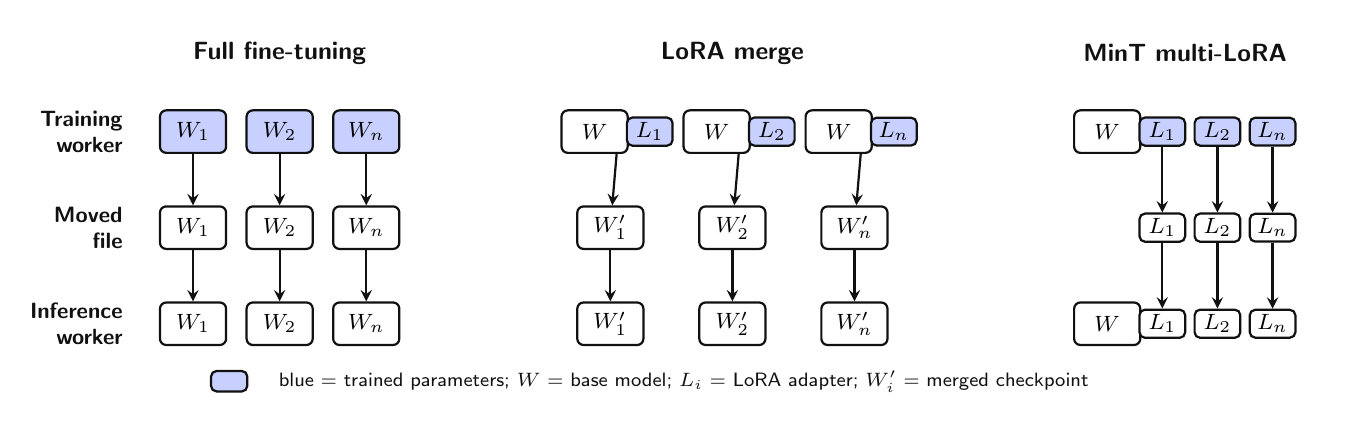
\begin{tikzpicture}[x=1cm,y=1cm,>=stealth,font=\footnotesize\sffamily]
  \tikzstyle{title}=[font=\bfseries\small\sffamily, text=mindlabfg, align=center]
  \tikzstyle{row}=[font=\bfseries\footnotesize\sffamily, text=mindlabfg, align=right]
  \tikzstyle{block}=[draw=mindlabfg, thick, rounded corners=0.8mm, fill=white, align=center, inner sep=2pt, minimum width=0.84cm, minimum height=0.54cm]
  \tikzstyle{trainblock}=[block, fill=mindlabblue!22]
  \tikzstyle{adapter}=[draw=mindlabfg, thick, rounded corners=0.7mm, fill=white, align=center, inner sep=1.8pt, minimum width=0.58cm, minimum height=0.34cm]
  \tikzstyle{trainadapter}=[adapter, fill=mindlabblue!22]
  \tikzstyle{note}=[font=\scriptsize\sffamily, text=mindlabfg, align=center]
  \tikzstyle{arrow}=[->, thick, draw=mindlabfg]

  \path[use as bounding box] (-1.45,-4.34) rectangle (14.95,0.42);

  \node[title] at (1.75,0.10) {Full fine-tuning};
  \node[title] at (7.50,0.10) {LoRA merge};
  \node[title] at (13.25,0.10) {MinT multi-LoRA};

  \node[row, anchor=east] at (-0.12,-0.90) {Training\\worker};
  \node[row, anchor=east] at (-0.12,-2.12) {Moved\\file};
  \node[row, anchor=east] at (-0.12,-3.34) {Inference\\worker};

  \foreach \x/\i in {0.65/1,1.75/2,2.85/n} {
    \node[trainblock] (ftw\i) at (\x,-0.90) {$W_{\i}$};
    \node[block] (ftc\i) at (\x,-2.12) {$W_{\i}$};
    \node[block] (fts\i) at (\x,-3.34) {$W_{\i}$};
    \draw[arrow] (ftw\i) -- (ftc\i);
    \draw[arrow] (ftc\i) -- (fts\i);
  }

  \foreach \x/\i in {5.95/1,7.50/2,9.05/n} {
    \node[block] (mb\i) at (\x-0.20,-0.90) {$W$};
    \node[trainadapter] (ml\i) at (\x+0.50,-0.90) {$L_{\i}$};
    \node[block] (mc\i) at (\x,-2.12) {$W'_{\i}$};
    \node[block] (ms\i) at (\x,-3.34) {$W'_{\i}$};
    \coordinate (join\i) at (\x+0.08,-1.18);
    \draw[arrow] (join\i) -- (mc\i);
    \draw[arrow] (mc\i) -- (ms\i);
  }
  \node[block] (mtw) at (12.26,-0.90) {$W$};
  \foreach \x/\i in {12.96/1,13.66/2,14.36/n} {
    \node[trainadapter] (mtl\i) at (\x,-0.90) {$L_{\i}$};
    \node[adapter] (mal\i) at (\x,-2.12) {$L_{\i}$};
    \draw[arrow] (mtl\i) -- (mal\i);
  }

  \node[block] (miw) at (12.26,-3.34) {$W$};
  \foreach \x/\i in {12.96/1,13.66/2,14.36/n} {
    \node[adapter] (msl\i) at (\x,-3.34) {$L_{\i}$};
    \draw[arrow] (mal\i) -- (msl\i);
  }

  \node[note] (legend) at (6.75,-4.07) {\quad blue = trained parameters; $W$ = base model; $L_i$ = LoRA adapter; $W'_i$ = merged checkpoint};
  \node[trainadapter, minimum width=0.46cm, minimum height=0.26cm, anchor=east] at (legend.west) {};
\end{tikzpicture}
}
    \caption{What crosses from training to serving under three adaptation paths. Blue marks the trained parameters. Full fine-tuning moves a full checkpoint for each variant. Merge-based LoRA trains adapters beside a resident base, then moves merged full checkpoints. MinT trains adapters beside a resident base and moves only adapter revisions to an inference engine that already holds the compatible base.}
    \label{fig:mint_handoff_paths}
\end{figure}

In this report, we introduce MinT's capabilities follow three scaling axes. \textit{Scale Up} supports LoRA RL on frontier-scale dense and MoE architectures, with model-parallel training and serving paths validated beyond 1T total parameters~\citep{qwen3_2025,deepseekv4_2026,glm5_2026,kimi_k2_2025}. This axis keeps the same adapter-revision path usable when the base requires tensor-parallel or expert-parallel placement, sparse-route consistency, and distributed adapter export. \textit{Scale Down} minimizes the training-serving handoff by moving only the exported LoRA adapter, which can be less than 1\% of the base-model size in compact rank-1 settings, eliminating full-checkpoint materialization entirely. In our measurements, adapter-only handoff reduces the measured handoff step by $18.3\times$ on a 4B dense model and by $2.85\times$ on a 30B MoE model; under the same resident-base allocation, concurrent multi-policy GRPO shortens wall time by $1.77\times$ and $1.45\times$, respectively, without increasing peak memory. \textit{Scale Out} expands the policy namespace while keeping engine-local execution bounded. MinT separates durable policy addressability from CPU/GPU hot working sets, builds on modern multi-adapter serving support~\citep{vllm2023,punica2024,slora2023,dlora2024,loraserve2025}, and treats first-touch adapter loading as scheduled service work. A tensor-parallel serving deployment supports $10^6$-scale addressable policy catalogs, with measured single-engine sweeps through 100K entries and thousand-adapter active waves at cluster scale; packed MoE LoRA tensors improve live engine loading by $8.5$--$8.7\times$ by reducing small-object fanout on the cold-load path. Together, these axes make continuously evolving LoRA post-training cheaper to operate, easier to reproduce, and better matched to multi-tenant policy populations.

MinT contributes four concrete pieces:

\begin{itemize}
    \item \textbf{Adapter lifecycle from update to serving.} MinT exports trained LoRAs as PEFT adapter revisions, including sharded-to-serving conversion, compatibility checks, rollout records, sampler loading, served-result attribution, and rollback. The adapter revision becomes the fixed behavior selected by rollout, evaluation, online serving, and recovery.

    \item \textbf{Large-scale multi-LoRA RL training.} MinT time-slices LoRA training sessions over resident shared bases and supports both single-worker PEFT and distributed Megatron training paths. It reports end-to-end LoRA RL on large dense and MoE deployments, including 235B-A22B-scale training and a 1T-class MoE countdown-task path.

    \item \textbf{Policy-population multi-LoRA serving.} MinT serves exported adapters through shared-base vLLM engines, separates durable policy addressability from CPU/GPU hot working sets, and treats cold loading as scheduled work for cache misses. Its packed MoE LoRA serving representation reduces small-object fanout and speeds live engine loading by 8.5--8.7$\times$.

    \item \textbf{Public reproducibility paths.} MinT provides a Tinker-compatible API~\citep{tinker2025,tinker_cookbook} and uses mint-cookbook recipes~\citep{mint_cookbook2026} to reproduce SFT, preference optimization, rollout-based RL, and AutoResearch examples through the same adapter lifecycle.
\end{itemize}

%%%


% 随着大语言模型进入更广泛的产品场景，用户对模型能力的需求持续上升，推动模型参数规模、后训练任务和生产部署流程不断扩张。模型规模的增长不仅意味着更高的算力消耗，也显著提高了训练与服务系统的整体复杂度：在硬件层面，系统需要管理大规模 GPU 集群，以及机房供电、散热、网络和资源调度等基础设施；在训练软件层面，系统需要协调分布式训练、任务编排、容错恢复、数据传输和推理服务；在模型工程层面，团队还需要维护模型版本、数据版本、实验分支、评测结果和回滚路径。尤其是在长程学习、工具使用和 agentic post-training 等场景中，训练、推理、环境交互和服务反馈被更紧密地耦合在一起，版本切换操作变得更加频繁和昂贵，使传统面向单个最终 checkpoint 的基础设施越来越难以支撑持续迭代。因此，LLM 后训练亟需一种更轻量、更可管理、也更用户友好的基础设施抽象。在实践中，LoRA 由于能够在冻结基础模型的同时，用小规模参数承载新的模型行为，被广泛认为是缓解这一复杂度的一条有潜力的路径。 



% MinT 正是围绕这一思路设计的基础设施系统。它并不把 LoRA 仅仅视为一种节省显存的训练技巧，而是将其提升为模型后训练中的基本策略单元：基础模型保持常驻，而具体的训练行为、产品分支、实验版本和回滚点则由不同的 LoRA adapter 承载。这样一来，系统在训练和服务之间不再需要频繁移动、加载或复制完整模型，而只需要传输和管理小规模的 LoRA 参数。进一步的，通过follow the practice of Tinker framework, MinT 将 rollout、参数更新、推理服务、版本导出和回滚等流程统一到一个以 LoRA 为中心的工作流中，并将底层复杂的分布式训练、模型切分、张量布局转换和服务接入隐藏在简洁的服务接口之后。通过这种方式，MinT 将训练更新和服务切换的操作工作在 LoRA adapter 上，避免频繁处理完整模型，从而降低多分支、多版本和多租户训练服务的系统复杂度。



% MinT 的能力可以从三个扩展维度来理解。

% 首先，**Scale Up** 关注模型规模的向上扩展，使 LoRA-based RL 能够运行在更大的 dense 和 MoE 架构之上，支持 Qwen、DeepSeek-style 等大模型家族，并在 GLM-5.1、Kimi K2 等前沿训练路径上进行验证。

% 其次，**Scale Down** 关注训练与服务之间的开销压缩。由于基础模型保持常驻，系统只需要在训练器和推理引擎之间传输 LoRA adapter，而不需要反复物化、搬移和加载完整 checkpoint。在极端情况下，rank-1 LoRA 的规模可以小到基础模型的约 1%，从而显著降低模型更新和服务切换成本。

% 最后，**Scale Out** 关注横向并发扩展。MinT 通过多级 adapter cache 同时管理和服务大量 LoRA 策略版本，使同一个基础模型之上可以承载多任务、多租户、多实验分支，乃至百万级 policy revisions。

% 通过这三个维度，MinT 不仅降低了单次训练或单次服务的成本，更将大规模、多版本、持续迭代的 LoRA 后训练转化为一种可管理、可复现、可扩展的基础设施能力。

% 基于上述设计，MinT 提供了三类核心系统能力。

% 第一，MinT 使超大模型上的 LoRA 强化学习训练更加可行。在大模型后训练中，多个实验分支往往需要共享同一个基础模型，但又各自维护不同的策略更新。MinT 通过让基础模型常驻，并在其上切换不同 LoRA adapter，使多个训练会话能够复用同一套底层模型资源。系统已验证其能够支持 Qwen3-235B-A22B 等大规模模型上的端到端 LoRA RL，并通过 Kimi K2 1T MoE 等更大规模部署路径进一步展示了这种架构的扩展潜力。

% 第二，MinT 降低了多版本 LoRA 在线服务的管理成本。在产品和实验场景中，同一个基础模型之上可能同时存在大量任务版本、用户分支或策略变体。MinT 将可被请求的 LoRA 名称目录、驻留在主机内存中的 LoRA 参数，以及正在 GPU 上服务的 LoRA adapter 分开管理，从而避免所有版本都同时占用昂贵的 GPU 资源。通过这种分层管理方式，系统能够支持大规模 LoRA 目录下的精确版本选择，并进一步推导出百万级 LoRA 版本管理的容量模型。

% 第三，MinT 提供了端到端的 基于LoRA 的后训练工作流，包含训练更新、服务发布、版本管理和实验复现。系统将训练得到的 LoRA adapter 作为独立版本进行管理，负责完成参数导出、格式转换、基础模型兼容性检查、服务接入、rollout 记录和版本回滚。同时，MinT 提供 Tinker-compatible API，并通过 mint-cookbook recipes 覆盖 SFT、preference optimization、rollout-based RL 和 AutoResearch 等典型任务，使用户能够在统一接口下复现和迁移不同类型的后训练实验。

\section{From LoRA Adapters to Managed Policy Revisions}

Once many trained behaviors share a few resident base models, MinT has to separate the bytes that execute a behavior from the service state that makes the behavior manageable. An \emph{adapter revision} is a fixed, exported snapshot of the LoRA adapter, frozen at a specific training step and stored in serving tensor layout; it is the executable LoRA payload that crosses from training to rollout, evaluation, and serving (it is not a training iteration or a transfer event). The policy record is the service-owned lifecycle state that makes that payload reproducible, reloadable, and rollbackable. This distinction lets a shared base support many LoRA policies without turning every policy into another full checkpoint or another full-model server.

An RL update leaves more than a LoRA file. After one update, the trainer has adapter tensors, optimizer moments, scheduler position, accumulated gradients, and rollout records that may still be needed for scoring. A sampler cannot consume that training checkpoint directly. It needs a fixed adapter revision in serving tensor layout, tied to the base model that is already resident in the inference engine. Later requests may select the same revision after the original worker has exited or after the serving cache has evicted the adapter bytes.

\begin{figure}[t]
\vspace{-0.7\baselineskip}
    \centering
    \resizebox{\linewidth}{!}{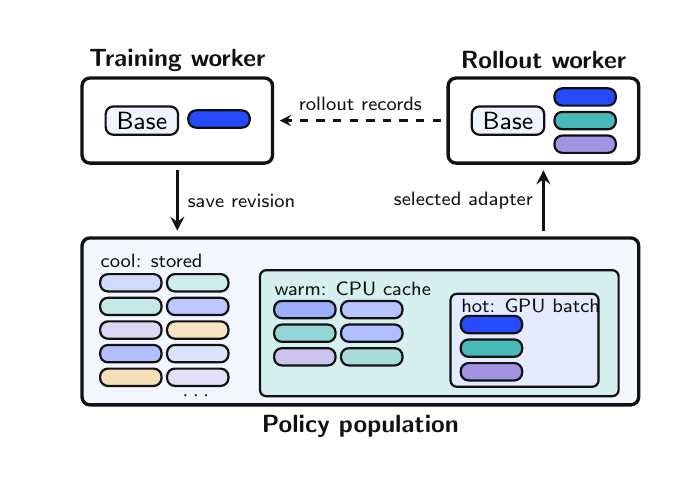
\begin{tikzpicture}[x=1cm,y=1cm,>=stealth,font=\small\sffamily]
  \definecolor{mintauxteal}{HTML}{009E9A}
  \definecolor{mintauxviolet}{HTML}{7057D2}
  \definecolor{mintauxamber}{HTML}{D98B00}
  \colorlet{loraone}{mindlabblue!85}
  \colorlet{loratwo}{mintauxteal!82}
  \colorlet{lorathree}{mintauxviolet!76}
  \colorlet{lorafour}{mindlabblue!58}
  \colorlet{lorafive}{mintauxamber!78}
  \colorlet{lorasix}{mindlabblue!38}
  \colorlet{loraseven}{mintauxteal!48}
  \colorlet{loraeight}{mindlabfg!30}
  \colorlet{coldtier}{mindlabbluepale!35}
  \colorlet{warmtier}{mintauxteal!16}
  \colorlet{hottier}{mindlabbluepale!78}
  \colorlet{coolone}{mindlabblue!18}
  \colorlet{cooltwo}{mintauxteal!24}
  \colorlet{coolthree}{mintauxviolet!24}
  \colorlet{coolfour}{mindlabblue!30}
  \colorlet{coolfive}{mintauxamber!28}
  \colorlet{warmone}{mindlabblue!38}
  \colorlet{warmtwo}{mintauxteal!42}
  \colorlet{warmthree}{mintauxviolet!36}
  \colorlet{warmfour}{mindlabblue!28}
  \colorlet{hotone}{mindlabblue!85}
  \colorlet{hottwo}{mintauxteal!72}
  \colorlet{hotthree}{mintauxviolet!64}
  \tikzstyle{frame}=[draw=mindlabfg, very thick, rounded corners=1mm, fill=white]
  \tikzstyle{tier}=[draw=mindlabfg, thick, rounded corners=0.8mm, fill=white]
  \tikzstyle{base}=[draw=mindlabfg, thick, rounded corners=1mm, fill=mindlabbluepale!45, align=center, inner sep=2pt, minimum width=0.92cm, minimum height=0.30cm]
  \tikzstyle{adapter}=[draw=mindlabfg, thick, rounded corners=1mm, minimum width=0.78cm, minimum height=0.22cm, inner sep=0pt]
  \tikzstyle{arrow}=[->, very thick, draw=mindlabfg, shorten >=2pt, shorten <=2pt]
  \tikzstyle{returnarrow}=[->, thick, dashed, draw=mindlabfg, shorten >=2pt, shorten <=2pt]
  \tikzstyle{title}=[font=\bfseries\small\sffamily, text=mindlabfg, align=center]
  \tikzstyle{label}=[font=\scriptsize\sffamily, text=mindlabfg, align=center, fill=white, inner sep=1.2pt]
  \tikzstyle{smalllabel}=[font=\scriptsize\sffamily, text=mindlabfg, align=center, fill=white, inner sep=1pt]
  \tikzstyle{plainlabel}=[font=\scriptsize\sffamily, text=mindlabfg, align=center, inner sep=1pt]
  \tikzstyle{tierlabel}=[font=\scriptsize\sffamily, text=mindlabfg, align=center, inner sep=0pt]

  \path[use as bounding box] (1.05,-3.18) rectangle (8.95,2.18);

  \node[frame, minimum width=2.42cm, minimum height=1.08cm] (trainer) at (2.95,1.00) {};
  \node[title] at (2.95,1.77) {Training worker};
  \node[base] at (2.50,1.00) {Base};
  \node[adapter, fill=hotone] at (3.48,1.02) {};

  \node[frame, minimum width=2.42cm, minimum height=1.08cm] (rollout) at (7.60,1.00) {};
  \node[title] at (7.60,1.77) {Rollout worker};
  \node[base] at (7.15,1.00) {Base};
  \node[adapter, fill=hotone] at (8.13,1.30) {};
  \node[adapter, fill=hottwo] at (8.13,1.00) {};
  \node[adapter, fill=hotthree] at (8.13,0.70) {};

  \node[frame, fill=coldtier, minimum width=7.07cm, minimum height=2.12cm] (population) at (5.275,-1.55) {};
  \node[tierlabel, anchor=west] at (1.97,-0.78) {cool: stored};
  \foreach \x/\y/\c in {
	    2.36/-1.06/coolone,2.36/-1.36/cooltwo,2.36/-1.66/coolthree,2.36/-1.96/coolfour,2.36/-2.26/coolfive,
	    3.21/-1.06/cooltwo!82,3.21/-1.36/coolfour!86,3.21/-1.66/coolfive!82,3.21/-1.96/coolone!74,3.21/-2.26/coolthree!76
  } {
    \node[adapter, fill=\c, minimum width=0.78cm] at (\x,\y) {};
  }
  \node[plainlabel] at (3.21,-2.50) {$\cdots$};

  \node[tier, fill=warmtier, minimum width=4.555cm, minimum height=1.60cm] (host) at (6.2775,-1.70) {};
  \node[tierlabel, anchor=west] at (4.18,-1.13) {warm: CPU cache};
  \foreach \x/\y/\c in {
	    4.57/-1.40/warmone,4.57/-1.70/warmtwo,4.57/-2.00/warmthree,
	    5.42/-1.40/warmfour,5.42/-1.70/warmone!82,5.42/-2.00/warmtwo!82
  } {
    \node[adapter, fill=\c, minimum width=0.78cm] at (\x,\y) {};
  }

  \node[tier, fill=hottier, minimum width=1.88cm, minimum height=1.18cm] (gpu) at (7.36,-1.79) {};
  \node[tierlabel, anchor=west] at (6.55,-1.35) {hot: GPU batch};
  \node[adapter, fill=hotone] at (6.94,-1.59) {};
  \node[adapter, fill=hottwo] at (6.94,-1.89) {};
  \node[adapter, fill=hotthree] at (6.94,-2.19) {};
  \node[title] at (5.275,-2.88) {Policy population};

  \draw[arrow] (trainer.south) -- node[label, right, pos=0.50, xshift=2pt] {save revision} (trainer.south |- population.north);
  \draw[arrow] (population.north -| rollout.south) -- node[label, left, pos=0.50, xshift=-2pt] {selected adapter} (rollout.south);
  \draw[returnarrow] (rollout.west) -- node[label, above, yshift=2pt] {rollout records} (trainer.east);
\end{tikzpicture}
}
    \caption{Adapter lifecycle in MinT. Training saves revisions into the policy population; rollout uses the hot GPU-batch subset and returns records for the next update.}
    \label{fig:policy_lifecycle}
    \vspace{-0.6\baselineskip}

\end{figure}

The service therefore has to answer four concrete questions after every update. Which base deployment can run this adapter? Which training checkpoint should a trainer restore if training resumes? Which fixed adapter revision should rollout, evaluation, or serving use? Where are those adapter bytes now: active in a GPU batch, cached in CPU memory, or only present in shared storage? MinT stores these answers separately because they change at different times.

A MinT policy record is the durable entry for one trained behavior over a compatible base model. It names the base version, LoRA rank and target modules, the latest training checkpoint, the rollout records kept for later updates, and the exported adapter revisions available for fixed behavior. A live training session is a temporary restoration of that record on a worker. MinT allows one training session per policy record; concurrent branches become separate records so each worker writes a different adapter and optimizer state. Export freezes the current training checkpoint into a fixed adapter revision. Evaluation, rollout, and online serving select a revision, while worker placement and cache state can change around it.

The RL loop crosses this lifecycle on every iteration. Rollout samples trajectories with a selected adapter revision on an inference engine that already holds the base. Training recomputes token probabilities for those trajectories, applies the objective, and changes the adapter and optimizer state. The next rollout needs another export because inference engines consume fixed PEFT adapter files in serving layout. Trainer-local optimizer checkpoints stay on the training side. Evaluation uses the same fixed-revision rule so a reported score names the adapter revision that produced it.

Serving adds another time scale. A request can name an adapter revision long after its bytes have left the local engine. The request first resolves a user-facing policy name to an exported revision and an engine-local adapter id. If the adapter is already active in the GPU batch, decoding can use it immediately. If it is cached in CPU memory, the engine promotes it. If it is absent from the local cache, the serving actor fetches the adapter file from shared storage and loads it before decoding. This lets MinT keep a large addressable catalog while bounding the much smaller CPU-cache and same-batch working sets.

Training has the opposite problem: one resident base deployment may serve several policy records over time. When a trainer switches from policy $A$ to policy $B$, MinT must save $A$'s adapter, optimizer moments, scheduler position, accumulated gradients, and unconsumed rollout records before restoring $B$'s corresponding state. The base weights stay resident. Only the LoRA tensors and training state change. Policies may also use different LoRA ranks or target-module sets, so the policy record carries the adapter shape that the worker must allocate and restore.

Sparse models split rollout metadata into two cases. MoE rollout records can carry selected expert ids. When the training backend can map those ids to its expert-parallel layout, log-probability scoring reuses the recorded expert path; when the ids are missing or unmappable, MinT removes that token from the replayed policy-gradient term. GLM-5-style dynamic sparse attention uses a different treatment. MinT currently lacks replay for every DSA indexer selection. The rollout record stores the backend/model path and correction policy, not per-token DSA indexer selections, and IcePop-style rollout correction zeroes importance weights whose training/rollout ratio falls outside the trusted band. That mitigation keeps unstable tokens out of the gradient term; it does not reconstruct the exact sparse-attention token set selected by the inference engine.

The adapter revision is the behavior-carrying payload; the policy record is the service state that makes that payload schedulable and durable. In this paper, a deployable LoRA policy over a resident base is the LLM behavior that MinT trains, evaluates, serves, and rolls back. MinT keeps the base deployment, training checkpoint, rollout record, exported adapter revision, and adapter cache state as separate facts so one trained behavior can be resumed, scored, exported, evicted, reloaded, and served in a larger population.

\section{System Design}
\label{sec:architecture}

MinT is a Tinker-compatible managed service for LoRA RL over resident base-model deployments. A client package calls the service to sample rollouts, compute gradients, apply an optimizer step, export an adapter revision, evaluate or serve that revision, and poll for the result. The service keeps the user-facing loop simple while dense and MoE bases remain loaded in resident trainers, samplers, and serving actors. Durable operation ids and policy records keep retries precise: the service knows which adapter generated a rollout, which checkpoint can resume training, which export is visible to samplers, and which resident worker can run the next request.

\Cref{fig:mint_overview} gives the service view, and \cref{fig:mint_handoff_paths} shows the training-serving boundary. The runtime must preserve both: a simple client interface and an adapter-only handoff. MinT therefore separates service control from resident compute. The service plane validates each call, records a pollable operation id, resolves the policy record or exported revision, and admits work onto a compatible worker. The compute plane has three service roles because different operations on one policy record require different compatible worker shapes. Single-worker PEFT trainers run LoRA updates when one worker can hold the base replica. Distributed Megatron trainer groups run LoRA updates when tensor, pipeline, or expert parallelism partitions the base and adapter tensors across ranks. vLLM sampler and serving actors hold inference bases and attach exported LoRA adapters for rollout, evaluation, and online serving. The runtime path has four mechanisms: service-plane visibility and policy-record resolution, time-sliced training over resident bases, export from trainer state to serving adapter files, and shared-base rollout or serving with adapter cache tiers.

\begin{figure}[tbp]
    \centering
    \resizebox{\textwidth}{!}{\usetikzlibrary{arrows.meta,calc,fit,positioning}
\colorlet{mintdark}{mindlabfg}
\colorlet{mintfill}{mindlabbluepale!45}
\begin{tikzpicture}[
    font=\sffamily\small,
    >=Latex,
    x=1cm,
    y=1cm,
    line cap=round,
    line join=round,
    panel/.style={
        draw=mintdark,
        very thick,
        rounded corners=3mm,
        fill=white
    },
    box/.style={
        draw=mintdark,
        thick,
        rounded corners=2mm,
        fill=mintfill,
        align=center,
        inner sep=3pt,
        minimum height=0.62cm
    },
    storagebox/.style={
        draw=black!55,
        thick,
        rounded corners=2mm,
        fill=white,
        align=center,
        inner sep=3pt,
        minimum height=0.50cm
    },
    patharrow/.style={
        ->,
        thick,
        draw=mintdark
    },
    softarrow/.style={
        ->,
        semithick,
        draw=black!50
    },
    botharrow/.style={
        <->,
        semithick,
        draw=black!50
    },
    statepath/.style={
        -,
        semithick,
        draw=black!45
    },
    metapath/.style={
        -,
        semithick,
        dashed,
        draw=black!50
    },
    label/.style={
        font=\sffamily\scriptsize,
        fill=white,
        inner sep=1pt,
        text=black!75,
        align=center
    },
    sublabel/.style={
        font=\sffamily\tiny,
        text=black!62,
        align=center
    },
    paneltitle/.style={
        font=\sffamily\bfseries\large,
        text=mintdark,
        fill=white,
        inner sep=2pt
    },
    storagetitle/.style={
        font=\sffamily\bfseries\normalsize,
        text=black!70,
        fill=white,
        inner sep=2pt
    },
    note/.style={
        font=\sffamily\scriptsize,
        text=black!65,
        align=center
    }
]

\path[use as bounding box] (-2.00,0.15) rectangle (20.80,5.92);

% =========================================================
% Top-level regions
% =========================================================

\node[
    box,
    minimum width=2.60cm,
    minimum height=1.35cm,
    text width=2.30cm
] (clients) at (-0.70,4.55) {
    MinT clients\\
    Tinker API
};

\draw[panel] (1.40,2.20) rectangle (10.70,5.65);
\node[paneltitle] at (6.05,5.65) {Service and control plane};

\draw[panel] (11.90,2.20) rectangle (17.40,5.65);
\node[paneltitle] at (14.65,5.65) {Compute plane};

\draw[
    draw=black!55,
    very thick,
    rounded corners=3mm,
    fill=mintfill
] (1.40,0.40) rectangle (17.40,1.55);

\node[storagetitle] at (9.40,1.55) {Durable storage};

% =========================================================
% Service and control plane
% =========================================================

\node[
    box,
    minimum width=1.25cm,
    minimum height=0.70cm
] (api) at (2.95,4.55) {
    API
};

\node[
    box,
    minimum width=1.35cm,
    minimum height=0.70cm
] (queue) at (4.72,4.55) {
    Queue
};

\node[
    box,
    minimum width=1.70cm,
    minimum height=0.88cm,
    text width=1.45cm
] (lookup) at (6.72,4.55) {
    Policy\\
    lookup
};

\node[
    box,
    minimum width=1.72cm,
    minimum height=0.88cm,
    text width=1.50cm
] (admit) at (8.91,4.55) {
    Resource\\
    admission
};

\node[
    box,
    minimum width=2.15cm,
    minimum height=0.70cm
] (future) at (6.05,3.15) {
    Operation state
};

% =========================================================
% Compute plane
% =========================================================

\node[
    box,
    minimum width=3.85cm,
    minimum height=0.90cm,
    text width=3.60cm
] (trainers) at (14.65,4.55) {
    PEFT / Megatron trainers
};

\node[
    box,
    minimum width=3.10cm,
    minimum height=0.90cm,
    text width=2.85cm
] (samplers) at (14.65,3.00) {
    vLLM samplers
};

% =========================================================
% Durable storage compartments
% =========================================================

\node[
    storagebox,
    minimum width=2.25cm
] (policy_store) at (3.80,0.88) {
    Policy records
};

\node[
    storagebox,
    minimum width=2.20cm
] (ckpt) at (7.55,0.88) {
    Checkpoints
};

\node[
    storagebox,
    minimum width=2.75cm
] (rollout) at (11.30,0.88) {
    Rollout records
};

\node[
    storagebox,
    minimum width=3.10cm
] (adapter) at (15.05,0.88) {
    Exported adapters
};

% =========================================================
% Request / admission path
% =========================================================

\draw[patharrow]
    (clients.east) -- (api.west);

\draw[patharrow] (api.east) -- (queue.west);
\draw[patharrow] (queue.east) -- (lookup.west);
\draw[patharrow] (lookup.east) -- (admit.west);

\draw[patharrow]
    (admit.east) -- (trainers.west);
\node[label] at (11.30,4.79) {schedule};

% =========================================================
% Operation state path through the API and compute result path
% =========================================================

\draw[botharrow]
    (api.south) |- (future.west);

\draw[softarrow]
    (11.90,3.15) -- node[label, above, pos=0.47] {result} (future.east);

% =========================================================
% Policy metadata and artifact paths
% =========================================================

\draw[softarrow]
    (trainers.south) -- (samplers.north);

\draw[botharrow]
    (14.65,2.20) -- node[label, right, pos=0.50] {state / artifacts} (14.65,1.55);

\draw[botharrow]
    (future.south) -- node[label, left, pos=0.68] {records} (6.05,1.55);

\end{tikzpicture}
}
\caption{MinT runtime organization. Tinker-compatible client packages call the service and receive a pollable operation id. The service queues the operation, reads the policy record, admits work onto the compute plane, and records completed operation results until clients poll them. Trainer workers update LoRA tensors and optimizer state over a resident base model; vLLM sampler and serving actors generate with exported adapter revisions. Durable storage holds checkpoints, rollout records, and exported revisions.}
    \label{fig:mint_architecture}
\end{figure}

\subsection{Service Plane and Resident Workers}

The service plane owns the client-visible state for each operation. It decides when a request becomes scheduled work, when a produced file becomes a usable checkpoint, exported revision, or result, and what a retry observes after a worker exits.

\paragraph{Operation visibility.}
The service plane turns each client call into scheduled work on a compatible resident worker. It validates the request, enqueues the operation, returns an id that the client can poll, and admits the work only when a worker with the required base deployment and adapter capacity is available. A worker may keep temporary tensors while it executes the call. A checkpoint, exported adapter revision, rollout record, or operation result becomes visible only when MinT writes the metadata entry that names its completed files and stores the pollable result. If a worker crashes after writing adapter files but before recording that entry, later requests cannot select those uncommitted files; the caller can retry the operation, and cleanup can remove unreferenced attempt paths. The same visibility rule covers training checkpoints, exported adapter revisions, rollout records, and pollable operation results.

\paragraph{Policy record resolution.}
Every training or sampling call resolves to a policy record before it reaches a worker. The record names the compatible base version, LoRA rank, target modules, and storage locations for checkpoints, rollout records, optimizer state, and exported revisions. Training restores the state named by the record: adapter tensors, optimizer moments, scheduler position, gradients, and rollout metadata. Sampling selects an exported adapter revision from the same record. If the service process restarts, completed checkpoints, exported revisions, rollout records, and finished operation results remain recoverable from storage.

\paragraph{Worker admission and eviction.}
Training and sampling workers consume cluster GPUs in different shapes, so the service admits them through one resource view. A single-worker PEFT trainer occupies one model replica. A Megatron training group spans tensor-parallel, pipeline-parallel, or expert-parallel ranks. A vLLM sampler reserves memory for a base model plus adapter slots. MinT tracks live workers, active training sessions, in-flight generation, pinned adapters, idle time, and reclaimable base deployments. Evicting an idle trainer frees compute while stored LoRA tensors, optimizer state, rollout records, and exported revisions remain requestable. Evicting an idle sampler removes actor-local cached adapters and GPU-batch slots while the exported revisions remain in shared storage for later loading.

\begin{figure}[H]
    \centering
    \resizebox{0.78\textwidth}{!}{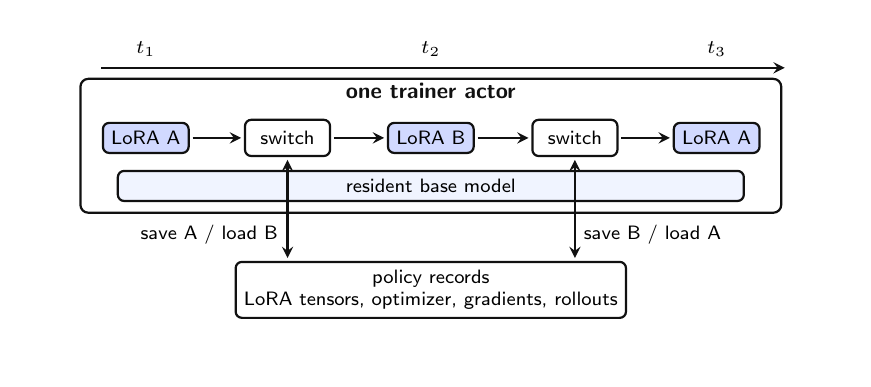
\begin{tikzpicture}[x=1cm,y=1cm,>=stealth,font=\scriptsize\sffamily]
  \tikzstyle{actor}=[draw=mindlabfg, thick, rounded corners=1mm, fill=white, align=center]
  \tikzstyle{base}=[draw=mindlabfg, thick, rounded corners=0.8mm, fill=mindlabbluepale!45, align=center, inner sep=3pt]
  \tikzstyle{slot}=[draw=mindlabfg, thick, rounded corners=0.8mm, fill=mindlabblue!18, align=center, inner sep=3pt]
  \tikzstyle{switch}=[draw=mindlabfg, thick, rounded corners=0.8mm, fill=white, align=center, inner sep=3pt]
  \tikzstyle{store}=[draw=mindlabfg, thick, rounded corners=0.8mm, fill=white, align=center, inner sep=3pt]
  \tikzstyle{arrow}=[->, thick, draw=mindlabfg, shorten >=1pt, shorten <=1pt]
  \tikzstyle{both}=[<->, thick, draw=mindlabfg, shorten >=1pt, shorten <=1pt]
  \tikzstyle{label}=[font=\scriptsize\sffamily, align=center, fill=white, inner sep=1pt]
  \tikzstyle{title}=[font=\bfseries\footnotesize\sffamily, align=center, text=mindlabfg]

  \path[use as bounding box] (-0.20,-2.35) rectangle (10.15,1.85);

  \draw[arrow] (0.70,1.34) -- (9.45,1.34);
  \node[label] at (1.30,1.58) {$t_1$};
  \node[label] at (4.92,1.58) {$t_2$};
  \node[label] at (8.55,1.58) {$t_3$};

  \node[actor, minimum width=8.90cm, minimum height=1.70cm] (trainer) at (4.92,0.35) {};
  \node[title] at (4.92,1.05) {one trainer actor};
  \node[base, minimum width=7.95cm, minimum height=0.36cm] (base) at (4.92,-0.16) {resident base model};

  \node[slot, minimum width=1.05cm, minimum height=0.38cm] (a1) at (1.30,0.45) {LoRA A};
  \node[switch, minimum width=1.08cm, minimum height=0.46cm] (sw1) at (3.10,0.45) {switch};
  \node[slot, minimum width=1.05cm, minimum height=0.38cm] (b2) at (4.92,0.45) {LoRA B};
  \node[switch, minimum width=1.08cm, minimum height=0.46cm] (sw2) at (6.75,0.45) {switch};
  \node[slot, minimum width=1.05cm, minimum height=0.38cm] (a3) at (8.55,0.45) {LoRA A};

  \node[store, minimum width=4.35cm, minimum height=0.62cm] (records) at (4.92,-1.48)
    {policy records\\\scriptsize LoRA tensors, optimizer, gradients, rollouts};

  \draw[arrow] (a1.east) -- (sw1.west);
  \draw[arrow] (sw1.east) -- (b2.west);
  \draw[arrow] (b2.east) -- (sw2.west);
  \draw[arrow] (sw2.east) -- (a3.west);

  \draw[both] (sw1.south) -- (records.north -| sw1.south);
  \node[label, anchor=east] at (3.02,-0.78) {save A / load B};
  \draw[both] (sw2.south) -- (records.north -| sw2.south);
  \node[label, anchor=west] at (6.82,-0.78) {save B / load A};
\end{tikzpicture}
}
    \caption{Time-sliced multi-LoRA training. One trainer keeps the base model resident. A scheduled policy loads its LoRA tensors, optimizer state, gradients, and rollout records into the trainer; the previous policy writes the same state back to storage before the switch.}
    \label{fig:mint_training_state_swap}
\end{figure}

\subsection{Time-Sliced Multi-LoRA Training}

MinT trains many LoRA policies over one resident base without allocating one base replica per policy. Replicating the frozen base for every active policy would spend most GPU memory on repeated weights and would remove the memory advantage that made LoRA attractive. Multi-LoRA training kernels, as explored by mLoRA for fine-tuning workloads~\citep{mlora2024}, can update several adapters in one batch. MinT instead time-slices policies on each trainer because RL requests usually contain enough rollout tokens to form efficient per-policy batches. The trainer swaps only the selected policy's LoRA tensors and optimizer state between requests while the frozen base remains loaded.

Each trainer time-slices locally. The service can run several resident trainers and samplers for the same base family, and the queue assigns ready policy operations across that pool. Each trainer executes one policy training session at a time so optimizer state and accumulated gradients have one writer, while other policies can progress on other workers or in sampler actors.

When policy $A$ yields the trainer to policy $B$, MinT writes $A$'s training state out and restores $B$'s state before the next gradient computation. The swapped state includes LoRA tensors, optimizer moments, scheduler position, accumulated gradients, and rollout records. After the update, MinT writes the changed state back. The base model stays in GPU memory across policy switches, while inactive adapter tensors and optimizer state can sit in CPU memory or storage until another request selects them.

The service supports different LoRA ranks and target-module sets on the same resident base when the worker was configured for those shapes. Two policies may use different ranks or target different modules, such as attention-only adapters versus adapters on attention, MLP, and output layers. A worker advertises supported adapter-shape limits when it joins the service. Within those limits, the trainer allocates adapter slots at configured maximum shapes, pads smaller adapters into those slots, and masks inactive rows or modules so each policy updates only its own parameters. Requests outside those limits require a worker configured for the larger rank or target-module set.

Single-worker PEFT trainers and distributed Megatron trainer groups restore LoRA tensors, run the update, and checkpoint the result. For smaller dense models, a trainer restores one adapter into one complete model replica. For Megatron MoE models, a trainer group restores tensor-parallel slices and expert-parallel adapter tensors onto the ranks that own the corresponding base shards. The model-parallel base remains distributed and resident; only LoRA tensors and optimizer state change when the scheduler selects a different policy.

\subsection{Adapter Data Flow Between Training and Serving}

After the trainer updates a LoRA, the next rollout, evaluation run, or serving request must use that adapter on an inference engine. The trainer holds LoRA tensors, optimizer state, and, for distributed training, rank-local tensor shards. vLLM expects a fixed adapter revision in the serving tensor layout, with optimizer state and rank-local training files removed. MinT exports the trained LoRA in PEFT format, carrying adapter tensors, rank, target modules, and base-model compatibility metadata without copying base checkpoint bytes.

Distributed export rebuilds serving adapter from sharded trainer files. Tensor-parallel ranks may hold slices of the same adapter tensor, and expert-parallel ranks may own different expert adapters. MinT gathers tensor-parallel slices, writes replicated tensors once, collects expert tensors from the ranks that own experts, and emits the PEFT layout expected by the sampler. For MoE adapters with shared-expert LoRA on each expert-parallel shard, the export path deduplicates shared-expert tensors, and the loader materializes one copy instead of repeating it for every shard. The file that crosses from training to rollout or serving is one adapter revision assembled in serving layout; it excludes merged base weights and rank-local training files.

The sampler admits an exported adapter only when its base model family, target modules, rank, and tensor layout match the resident base deployment and configured adapter buffers. The policy may continue training after export, while evaluation and serving select the fixed revision produced by a particular export.

\begin{figure}[H]
    \centering
    \resizebox{0.84\textwidth}{!}{\begin{tikzpicture}[x=1cm,y=1cm,>=stealth,font=\footnotesize\sffamily]
  \tikzstyle{actor}=[draw=mindlabfg, very thick, rounded corners=1mm, fill=white]
  \tikzstyle{box}=[draw=mindlabfg, thick, rounded corners=0.8mm, fill=mindlabbluepale!45, align=center, inner sep=4pt]
  \tikzstyle{store}=[draw=mindlabfg, thick, rounded corners=0.8mm, fill=white, align=center, inner sep=4pt]
  \tikzstyle{slotbox}=[draw=mindlabfg, thick, rounded corners=0.8mm, fill=white, align=center, inner sep=3pt]
  \tikzstyle{adapter}=[draw=mindlabfg, thick, rounded corners=1mm, align=center, minimum width=0.86cm, minimum height=0.23cm, inner sep=0pt, fill=mindlabfg!8]
  \tikzstyle{selected}=[draw=mindlabfg, thick, rounded corners=1mm, align=center, font=\scriptsize\sffamily, minimum width=1.14cm, minimum height=0.30cm, inner sep=1.2pt, fill=mindlabblue!38]
  \tikzstyle{arrow}=[->, very thick, draw=mindlabfg, shorten >=2pt, shorten <=2pt]
  \tikzstyle{hot}=[->, very thick, draw=hotpath, shorten >=2pt, shorten <=2pt]
  \tikzstyle{cold}=[->, thick, dashed, draw=coldpath, shorten >=2pt, shorten <=2pt]
  \tikzstyle{label}=[font=\footnotesize\sffamily, align=center, fill=white, inner sep=1.5pt, text=mindlabfg]
  \tikzstyle{smalllabel}=[font=\scriptsize\sffamily, align=center, fill=white, inner sep=1.1pt, text=mindlabfg]
  \tikzstyle{title}=[font=\bfseries\footnotesize\sffamily, align=center, text=mindlabfg]
  \colorlet{hotpath}{mindlabblue}
  \colorlet{coldpath}{mindlabline}

  \path[use as bounding box] (0.20,-2.42) rectangle (14.05,2.18);

  \node[box, minimum width=1.92cm, minimum height=0.72cm] (map) at (2.92,0.40) {Serving map\\policy $\to r$};

  \node[actor, minimum width=7.02cm, minimum height=3.70cm] (actor) at (8.53,-0.18) {};
  \node[title] at (8.53,1.44) {vLLM sampler actor};

  \node[slotbox, minimum width=1.86cm, minimum height=1.28cm] (gpu) at (6.64,0.40) {};
  \node[smalllabel, anchor=south] at (6.64,1.09) {GPU LoRA slots};
  \node[adapter] at (6.64,0.72) {};
  \node[selected] (selected) at (6.64,0.40) {$L_r$};
  \node[adapter] at (6.64,0.08) {};

  \node[box, minimum width=2.10cm, minimum height=0.76cm] (infer) at (10.30,0.40)
    {vLLM\\generation};
  \node[store, minimum width=2.10cm, minimum height=0.78cm] (base) at (10.30,-1.35)
    {resident\\model};
  \node[label, anchor=west] (tokens) at (12.54,0.40) {response tokens};

  \node[store, minimum width=1.86cm, minimum height=0.78cm] (warm) at (6.64,-1.35)
    {CPU adapter\\cache};
  \node[store, minimum width=2.50cm, minimum height=0.78cm] (catalog) at (2.63,-1.35)
    {shared adapter\\storage};

  \draw[arrow] (0.62,0.40) -- node[smalllabel, above, pos=0.42] {request} (map.west);
  \draw[hot] (map.east) -- node[smalllabel, above, yshift=3pt, pos=0.50, text=hotpath] {hit: $L_r$ resident} (gpu.west);
  \draw[hot] (gpu.east) -- node[smalllabel, above, yshift=3pt, pos=0.50, text=hotpath] {selected $L_r$} (infer.west);
  \draw[arrow] (base.north) -- (infer.south);
  \draw[arrow] (infer.east) -- (tokens.west);

  \draw[cold] (catalog.east) -- node[smalllabel, above, pos=0.50, text=coldpath] {fetch $r$} (warm.west);
  \draw[cold] (warm.north) -- node[smalllabel, right, xshift=6pt, pos=0.44, text=coldpath] {admit $L_r$} (gpu.south);

  \draw[hot, -] (12.42,-1.09) -- (12.88,-1.09);
  \node[smalllabel, anchor=west, text=hotpath] at (12.94,-1.09) {hot path};
  \draw[cold, -, dashed] (12.42,-1.61) -- (12.88,-1.61);
  \node[smalllabel, anchor=west, text=coldpath] at (12.94,-1.61) {cold path};
\end{tikzpicture}
}
\caption{Shared-base multi-LoRA sampling. A request reaches the serving map, which resolves the selected policy to exported adapter revision $r$. The solid path uses revision $r$ because its LoRA $L_r$ is already in a GPU batch slot. The vLLM actor runs inference with the resident base and $L_r$, then returns response tokens. Dashed arrows show the cold path: fetch revision $r$ from shared storage into the per-sampler CPU cache, then admit $L_r$ into a GPU batch slot before inference.}
    \label{fig:mint_system_blocks}
\end{figure}

\subsection{Shared-Base Rollout and Serving}

MinT uses vLLM for rollout and serving because vLLM can run inference from a resident base with a LoRA adapter resident in a GPU batch slot. vLLM handles token generation. MinT handles revision selection, adapter load queues, adapter cache tiers, and the export path that turns trainer state into serving adapter files. A sampler actor keeps one base deployment resident, admits exported adapters into vLLM's LoRA slots, and runs inference with the adapter named by MinT. The service maps a user-facing policy name to a policy record, chooses an exported adapter revision, and sends the sampler that revision. \Cref{fig:mint_system_blocks} shows the serving path for a request that resolves to revision $r$.

Each sampler manages adapter cache state across three tiers, which \cref{sec:e4_serving} measures in detail. The addressable catalog holds exported revisions in shared storage. The CPU cache holds adapter bytes already near one sampler actor. The GPU batch holds adapters resident in current inference slots. A request uses a GPU-batch adapter if it is already resident in a slot, promotes a CPU-cached adapter if it is warm, or schedules a cold load from shared storage if the adapter is only in the catalog. Cold adapter loads are scheduled service work before inference: MinT resolves the revision, queues the load job, controls which cold loads enter the sampler, and delays inference starts when too many distinct cold adapters arrive together.

\section{Three Scaling Axes}
\label{sec:scaling}

\Cref{sec:architecture} defined the training-to-serving path: a rollout is generated by a resident base plus an adapter revision, training updates that adapter, and export returns a PEFT adapter file in serving layout. Scaling MinT stresses three parts of that path: large-base placement, exported adapter bytes, and adapter cache state. \textbf{Scale up} keeps LoRA RL usable when dense or MoE bases require model-parallel placement and sparse-routing metadata. \textbf{Scale down} makes the adapter revision, rather than a merged checkpoint, the object that crosses from training to serving. \textbf{Scale out} keeps a large addressable policy catalog selectable while each engine admits only bounded CPU-resident and GPU-active working sets.

\subsection{Scale Up: LoRA RL on Large Dense and MoE Bases}

\paragraph{Megatron placement.}
MinT uses Megatron training groups when the base model is too large for a single PEFT worker. Tensor parallelism shards dense tensors. Expert parallelism assigns MoE experts to rank groups. Dense-module LoRA tensors follow the tensor-parallel shards for the dense weights they modify. Per-expert LoRA tensors are keyed by expert id: the EP shard owns the experts assigned to it, and TP shards the expert matrices inside that owner group when the run also uses tensor parallelism. Shared-expert LoRA is stored once per EP shard and deduplicated during export.

\paragraph{Policy switching.}
The base shards stay resident across policies. A policy switch restores the adapter tensors, optimizer moments, and accumulated gradients on the ranks that will execute the next update. This keeps the policy training state small relative to the resident base while preserving Megatron's sharding rules.

\paragraph{Distributed export.}
Serving needs one PEFT adapter revision that can attach to a resident vLLM base deployment. Export converts the Megatron training view into that serving view: tensor-parallel LoRA slices are gathered, replicated tensors are deduplicated, and expert LoRA tensors are collected from their expert-parallel owners. The exported adapter is the policy revision that later appears in serving, evaluation, rollback, and catalog records.

\paragraph{MoE router replay.}
MoE RL requires training-time scoring to use the expert path that generated each rollout token. R3 identifies router mismatch as a concrete source of instability in MoE RL: small implementation or precision differences can route the same token to different experts during rollout and training~\citep{r3_moe_router2025,chiang2026routerreplay}. R3 records MoE expert routing. For Qwen3-style MoE runs, MinT stores selected expert ids with rollout records. Training can replay a recorded route when the backend can reconstruct that expert path. Training masks a token when the rollout record lacks selected expert ids or the training backend cannot map those ids to its expert-parallel layout.

\paragraph{Sparse-attention provenance.}
Dynamic sparse attention has a separate mismatch channel. In GLM-5 and GLM-5.1, the DSA indexer and top-$k$ path decide which tokens participate in sparse attention; small numerical differences can change that token set~\citep{glm5_2026,stevenchiang2026supportglm5inmint}. MinT removes observed implementation mismatches where the stack exposes a concrete cause: indexer RoPE layout, normalized query/key inputs, deterministic top-$k$ behavior, frozen indexer defaults, long-context THD/CP support, and LoRA loading for DSA target modules. Probability mismatch can remain after those fixes, so MinT uses IcePop-style rollout correction~\citep{ling_every_step2025}: when the training/rollout probability ratio leaves the configured lower--upper trusted band, the token receives zero importance weight. This mitigation filters unsafe scoring terms. It does not replay every DSA indexer choice, and it does not prove that training used the exact sparse-attention token set selected by the inference engine.

\begin{table}[H]
\centering
\scriptsize
\setlength{\tabcolsep}{4pt}
\renewcommand{\arraystretch}{1.20}
\caption{Representative model-family support validated by the current MinT stack.}
\label{tab:supported_model_families}
\fittowidth{%
\begin{tabular}{@{}M{0.16\textwidth}M{0.18\textwidth}M{0.28\textwidth}M{0.32\textwidth}@{}}
\toprule
\apphead Family & Model structure & Scale validated & MinT support path \\
\midrule
\appkey{Qwen3 series} & Dense and MoE variants & 0.6B/4B dense adapters; 30B-A3B and 235B-A22B MoE runs & Single-worker PEFT, Megatron MoE training, expert-route records, adapter export, and shared-base serving \citep{qwen3_2025,chiang2026routerreplay} \\
\addlinespace[3pt]
\appkey{Moonlight \& Kimi K2} & MLA MoE & Moonlight-16B-A3B bring-up; Kimi K2 1.04T countdown-task LoRA RL & MLA/MoE adapter placement, Megatron-Bridge conversion, vLLM serving, and trillion-parameter-class LoRA RL \citep{chiang2026routerreplay,liu2025Build,kimi_k2_2025} \\
\addlinespace[3pt]
\appkey{GLM-5 / GLM-5.1} & MLA, DSA, MTP, and MoE & Frontier agentic family with DSA/MTP training and serving bring-up & DSA/MTP training patches, DSA LoRA target mapping, vLLM custom-forward LoRA loading, bridge conversion, and IcePop rollout correction \citep{glm5_2026,stevenchiang2026supportglm5inmint,ling_every_step2025} \\
\bottomrule
\end{tabular}%
}
\end{table}


\subsection{Scale Down: Adapter-Only Training-Serving Handoff}

\paragraph{Adapter handoff bytes.}
The training-serving handoff uses the LoRA adapter as the checkpoint. A measured Qwen3-4B rank-32 PEFT adapter file is 264{,}310{,}274 bytes, about 252 MiB. Adapter byte size is determined by rank, target modules, dtype, and tensor layout. A four-billion-parameter bf16 base checkpoint has an 8.0 GB weight floor before metadata and optimizer state. The measured adapter is about 3.3\% of that base-weight floor, and the serving path can load it without materializing another full base copy. Since LoRA tensor bytes scale approximately linearly with rank for a fixed target-module set, the same target pattern at rank 1 would be about 7.9 MiB, or roughly 0.10\% of the bf16 base-weight floor. This supports the abstract's conservative 1\% claim: compact rank-1 settings can fall below 1\%, while broader target-module choices and metadata can increase the footprint. The system property remains the same: the crossing artifact is an adapter revision, not a full checkpoint.

\paragraph{Serving-compatible export.}
MoE export applies the same adapter-revision rule to sharded training runs. The trainer writes a PEFT adapter file in the tensor layout expected by vLLM, with optimizer state and rank-local training files removed. The file that crosses from training to serving is the adapter revision.

\paragraph{Served-score attribution.}
A served score names the exported adapter revision together with its compatible base model, target modules, prompt renderer, scorer, and serving path. When a row reports a served score, MinT compares isolated adapter loading against shared-base serving before attributing the served score to the exported revision. This check separates the policy result from loader and routing differences.

\subsection{Scale Out: Policy-Population Serving}
\label{sec:scale_out_residency}

\paragraph{From stored adapters to live policies.}
Scale-out begins when exported adapters stop being a small set of training files and become a large set of deployable policies. The catalog can grow with tenants, product variants, rollback points, personalization branches, evaluation snapshots, and research sweeps. A user-facing name resolves to an exported adapter revision, the revision resolves to a durable adapter file, and a serving actor maps that file to a local adapter id when the policy enters that actor. \Cref{tab:scale_out_cache_tiers} names the three tiers that a policy revision can occupy at once; the paragraphs below visit them in turn.

\begin{table}[t]
\centering
\scriptsize
\setlength{\tabcolsep}{3.2pt}
\renewcommand{\arraystretch}{1.10}
\caption{Three cache tiers separate addressability from local residency and same-batch execution. A policy revision can occupy any subset of these tiers at a given moment; the scales, lifetimes, and control surfaces differ.}
\label{tab:scale_out_cache_tiers}
\fittowidth{%
\begin{tabular}{@{}M{0.16\textwidth}M{0.15\textwidth}M{0.15\textwidth}M{0.22\textwidth}M{0.26\textwidth}@{}}
\toprule
\apphead Tier & Scale & Lifetime & Promotion / eviction & Measured in this paper \\
\midrule
\appkey{Addressable catalog} & $10^3$--$10^6$ entries & Durable (control plane) & Promoted by adapter export; retired manually & Catalog sweep 1k--100k (\cref{tab:e4_serving_summary}); $10^6$-entry sizing in Appendix~\cref{tab:app_fleet_model} \\
\addlinespace[3pt]
\appkey{CPU adapter cache} & Hundreds per engine & Per actor run & Promoted by router or cache-miss load; LRU under memory pressure & 369 / 550 cached on one engine (\cref{tab:e4_serving_summary}; Appendix~\cref{tab:app_cache_ladders}) \\
\addlinespace[3pt]
\appkey{GPU batch} & $\le 64$ distinct adapters & One decoding step & Promoted by the batch scheduler; released at end of step & Same-batch frontier $N{=}64$ (\cref{tab:e4_serving_summary}; Appendix~\cref{tab:app_cache_ladders}) \\
\bottomrule
\end{tabular}%
}
\end{table}

\paragraph{Catalog size is the request-name scale.}
The measured 1k--100k catalog sweep keeps name resolution separate from engine-local cache state. The Qwen3-30B TP=4 experiments resolve request names against catalogs up to 100k entries, keep hundreds of adapters cached near one engine, and run clean same-batch probes through 64 distinct adapters. Appendix~\cref{tab:app_fleet_model} extrapolates the measured single-engine limits to a $10^6$-entry accumulated catalog under a fleet-level routing model. These measurements split scale-out into three quantities: how many policy revisions can be named, how many can stay cached near an engine, and how many can execute in the current batch. The $10^6$ number is addressability, not simultaneous GPU residency.

\paragraph{Traffic locality drives cache state.}
Catalog membership and local cache state change on different time scales. Catalog entries live in the control plane. Cache entries are local to a serving actor. The same adapter revision can be addressable in the catalog, cached in CPU memory on one actor, active in the current GPU batch, evicted back to shared storage, and later loaded again. Recurring traffic should stay near an engine that already holds the selected policy, while weak-locality sweeps and rollout waves expose cache misses.

\paragraph{Cold loading is service work.}
A cache miss does more than read a small LoRA file. The serving actor fetches tensors, materializes loader objects, registers the adapter with the engine, and activates it before decoding can start. Different missing policies serialize through the engine load path, so latency grows as a staircase when many unique policies arrive together. Concurrent cache-miss requests for the same missing policy can share one load; requests for different missing policies remain separate load jobs. MinT therefore treats cold loading as scheduled service work with deduplication and bounded backpressure.

\paragraph{Serving contract.}
Policy-population serving requires controls after name lookup. Routing preserves CPU-cache reuse when traffic has locality. Batch construction respects the smaller same-batch adapter limit; the addressable catalog is larger than any realized batch. Cold loading is observable, retryable, and backpressured because it turns a stored adapter revision into an engine-local adapter object. The policy record and exported revision stay stable while the adapter moves among shared storage, the CPU cache, and the GPU batch.

\paragraph{Representation controls the load staircase.}
MoE LoRA makes the cold path visible because a moderate-size adapter can expand into tens of thousands of tiny tensor objects and hundreds of megabytes of cached state across TP workers. MinT packs these tensors into a serving representation with nearly unchanged declared bytes, reducing object fanout before engine registration. The detailed serving measurements in \cref{sec:e4_serving} show 37{,}248 tensors reduced to 672 and an 8.5--8.7$\times$ live-load speedup, with the packed live engine-load slice below 0.2 seconds in the measured bursts. This live-load number is one component of a longer cold path that also includes routing, queueing, fetch, and generation. The exported adapter remains the policy unit, while cold loading becomes an explicit adapter lifecycle stage that can be routed, prewarmed, throttled, and optimized.

\section{Evaluation}
\label{sec:evaluation}

\begin{figure}[H]
    \centering
    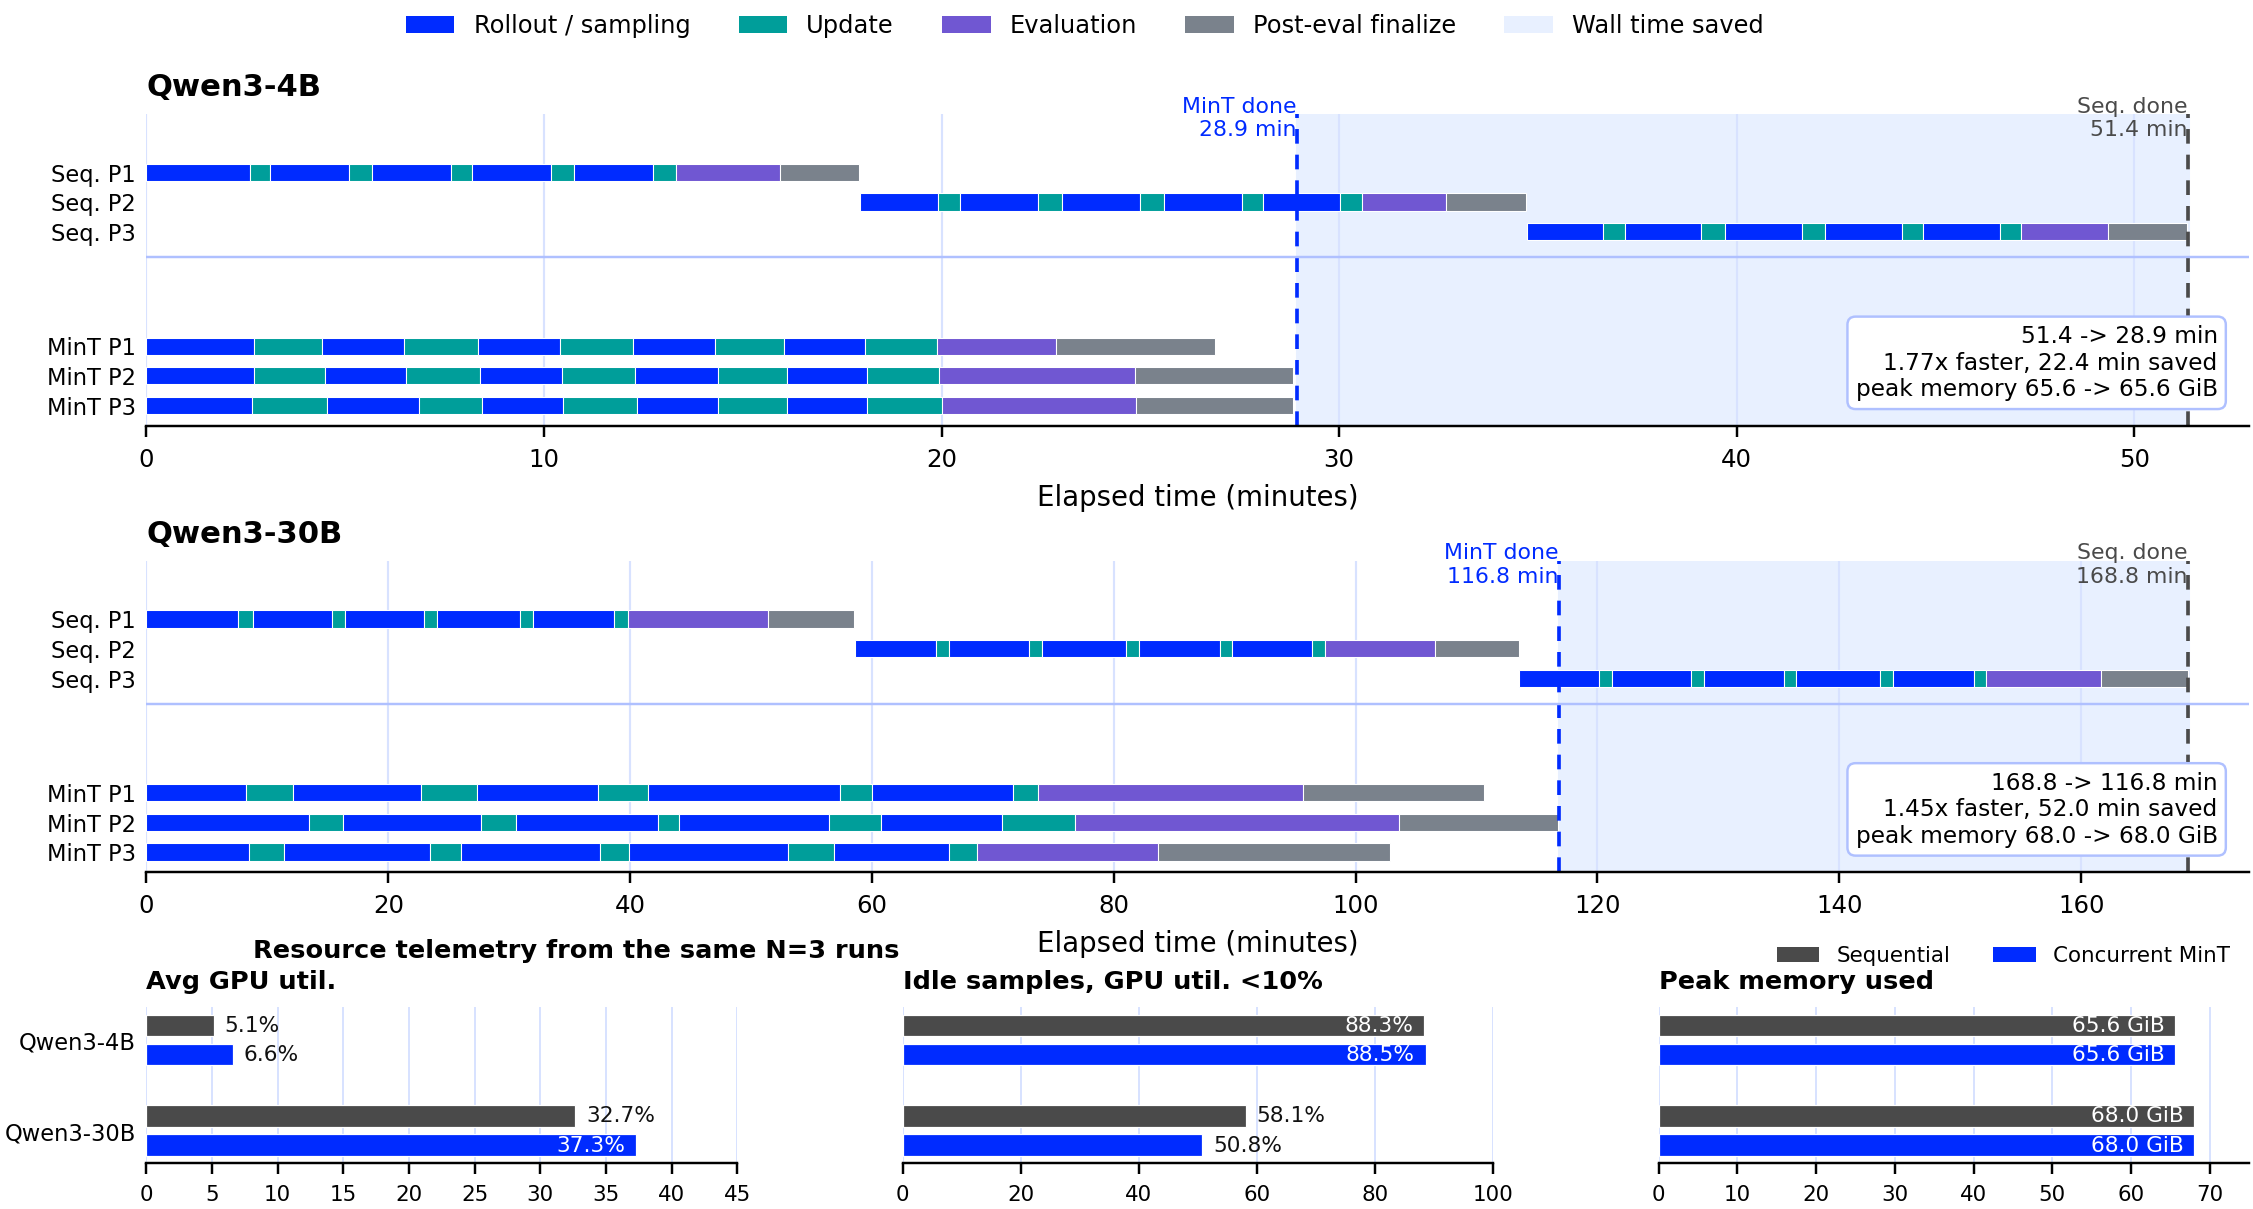
\includegraphics[width=\textwidth]{figures/eval_n3_schedule_timeline.png}
    \caption{Concurrent multi-LoRA training overlaps GRPO runs under the same base-model allocation. Timeline lanes show the schedule, and the lower panels summarize average GPU utilization, samples below 10\% utilization, and peak memory from the same runs. Vertical dashed lines mark completion time for the concurrent and sequential schedules.}
    \label{fig:e2_gpu_utilization}
\end{figure}

\begin{table}[H]
\centering
\scriptsize
\setlength{\tabcolsep}{3.2pt}
\renewcommand{\arraystretch}{1.10}
\caption{Concurrent-training schedule summary for three GRPO policies. Time saved and speedup compare each concurrent MinT row against the sequential row for the same model.}
\label{tab:e2_training_utilization}
\fittowidth{%
\begin{tabular}{@{}M{0.14\textwidth}M{0.19\textwidth}M{0.16\textwidth}M{0.15\textwidth}M{0.19\textwidth}M{0.10\textwidth}M{0.13\textwidth}@{}}
\toprule
\apphead Model & Schedule & Workloads & Wall time & Time saved & Speedup & Peak memory \\
\midrule
\appgroup{7}{Qwen3-4B}
Qwen3-4B & \appkey{Sequential} & 3 GRPO policies & 3081.2 s & -- & $1.00\times$ & 65.6 GiB \\
Qwen3-4B & \appkey{Concurrent MinT} & 3 GRPO policies & 1736.1 s & 1345.1 s / 43.7\% & $1.77\times$ & 65.6 GiB \\
\appgroup{7}{Qwen3-30B}
Qwen3-30B & \appkey{Sequential} & 3 GRPO policies & 10130.0 s & -- & $1.00\times$ & 68.0 GiB \\
Qwen3-30B & \appkey{Concurrent MinT} & 3 GRPO policies & 7008.4 s & 3121.6 s / 30.8\% & $1.45\times$ & 68.0 GiB \\
\bottomrule
\end{tabular}%
}
\end{table}

The experiments test the three scaling axes through the same LoRA lifecycle. Scale Down is measured by adapter-only handoff against merge-and-load paths and by concurrent training schedules that reuse one resident base allocation. Scale Up is measured by dense SFT, DPO, and GRPO runs, sparse-route MoE RL, Qwen3-235B-A22B GRPO, and a Kimi K2 1T countdown-task path. Scale Out is measured by separating addressable catalog size, CPU-cache size, same-batch adapter diversity, and cold-load cost; the million-scale claim is a catalog and routing claim, not a claim that one engine keeps every adapter resident or active.

An adapter revision means a fixed exported adapter version selected by rollout, evaluation, serving, or rollback. The term names the behavior selected by a request, separate from the file transfer or load operation that may place that adapter near a sampler.

The handoff and utilization measurements isolate the systems effect of making the adapter the training-serving artifact. The learning measurements confirm that the same lifecycle supports the public cookbook recipes and larger sparse-model deployments. The serving measurements show that a large policy catalog is an addressability scale, while CPU-cache residency, same-batch adapter diversity, and cold-load work are the online execution scales. This distinction is the evidence boundary for the abstract: MinT can manage a million-scale catalog while training and serving selected revisions through bounded resident working sets.

SFT denotes supervised fine-tuning. DPO denotes pairwise preference optimization. GRPO denotes rollout-based reinforcement learning. The public MinT cookbook is the recipe layer around the framework: it packages task configurations, benchmark manifests, proxy screens, full confirmations, and maintained adapter recipes~\citep{mint_cookbook2026}. DAPO-AIME24 is the math-RL cookbook recipe evaluated on AIME 2024, chat-DPO is the pairwise-preference recipe, LawBench is the legal-reasoning recipe, and Fineval is a finance-domain supervised benchmark.

\begin{figure}[H]
    \centering
    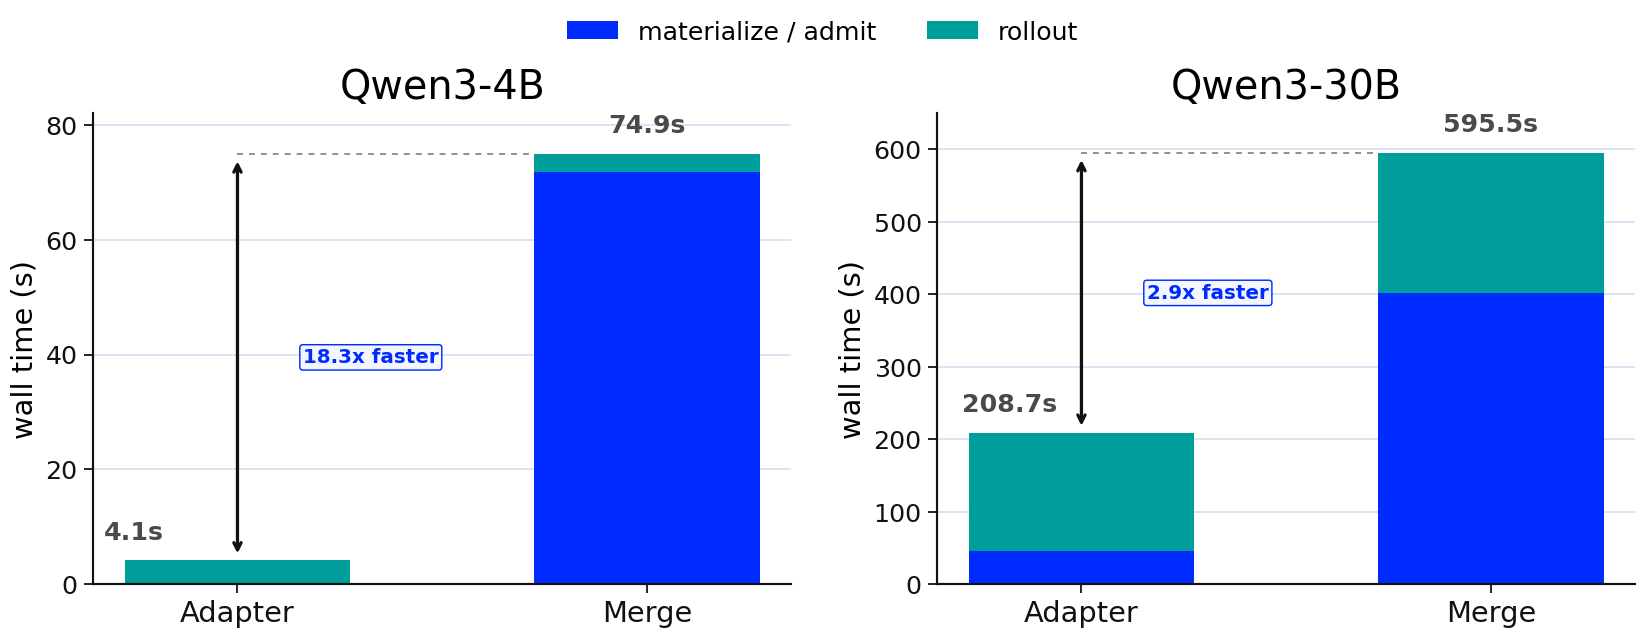
\includegraphics[width=0.92\textwidth]{figures/eval_handoff_breakdown.png}
    \caption{Adapter handoff avoids the merge-and-load stages that dominate the full-checkpoint path. Each stacked bar separates materialization or adapter loading from rollout under the probe protocol for the corresponding model.}
    \label{fig:e1_handoff_breakdown}
\end{figure}
\subsection{Scale Down and Multi-Train Utilization}
\label{sec:e12_pilots}

Adapter handoff compares two ways to send a newly trained policy to the sampler. The merge path materializes a full checkpoint and then loads that checkpoint before rollout. The MinT path loads the exported adapter into a resident shared-base sampler. \Cref{fig:e1_handoff_breakdown} plots total step time as materialization or adapter loading plus rollout, and \cref{tab:e1_handoff_paths} records the file sizes, cold first-sample latency, and total versus warm generation rates used to interpret the bars. The total rate includes the first request in the probe sequence, while the warm rate excludes it. A merged checkpoint may achieve higher or lower token throughput than a LoRA-based adapter during rollout, so the end-to-end comparison involves a trade-off between the cost of shipping the artifact and the resulting sampling throughput. In these runs, loading the adapter saves enough materialization and loading time to dominate the rollout-speed differences.

\begin{table}[H]
\centering
\scriptsize
\setlength{\tabcolsep}{3pt}
\renewcommand{\arraystretch}{1.05}
\caption{File and sampling metrics for the adapter-handoff comparison in \cref{fig:e1_handoff_breakdown}. Cold first sample is the first request wall time. The total sample speed includes that first request, while the warm sample speed excludes it.}
\label{tab:e1_handoff_paths}
\fittowidth{%
\begin{tabular}{@{}M{0.11\textwidth}M{0.12\textwidth}M{0.16\textwidth}M{0.14\textwidth}M{0.17\textwidth}M{0.13\textwidth}M{0.15\textwidth}@{}}
\toprule
\apphead Model & Path & Checkpoint parameters & Checkpoint file size & Materialization or load & Cold first sample & \makecell{sample speed\\total/warm} \\
\midrule
\appgroup{7}{Qwen3-4B}
Qwen3-4B & \appkey{Adapter} & rank-32 LoRA & 252 MiB & 0.036 s & 4.114 s & 15.568/15.567 tok/s \\
Qwen3-4B & \appkey{Merge} & full model & 8.061 GB & 71.820 s & 55.704 s & 4.697/20.595 tok/s \\
\appgroup{7}{Qwen3-30B}
Qwen3-30B & \appkey{Adapter} & rank-16 LoRA & 1.692 GB & 46.455 s & 117.304 s & 1.874/5.700 tok/s \\
Qwen3-30B & \appkey{Merge} & full model & 61.084 GB & 402.245 s & 156.074 s & 1.573/6.904 tok/s \\
\bottomrule
\end{tabular}%
}
\end{table}

Concurrent training measures schedule utilization under one resident base allocation. A sequential schedule can fit in memory while leaving the resident base idle between rollout, update, export, and evaluation phases. MinT keeps the same peak memory budget and lets other policies use those idle periods on resident trainers and samplers. The measured speedup comes from filling cross-policy gaps in the schedule, while each rollout and optimizer step still runs the same model computation for its selected policy. In the completed GRPO runs, concurrent execution finishes in 1736.1 s instead of 3081.2 s on Qwen3-4B and in 7008.4 s instead of 10130.0 s on Qwen3-30B, while peak memory remains unchanged within each model size. \Cref{fig:e2_gpu_utilization} shows the measured schedule timeline and matching GPU telemetry, and \cref{tab:e2_training_utilization} records the schedule summaries.

The timing and utilization experiments isolate the systems effect of the adapter design. Learning quality is evaluated under the same adapter lifecycle in the next group of experiments.
\FloatBarrier

\begin{figure}[H]
    \centering
    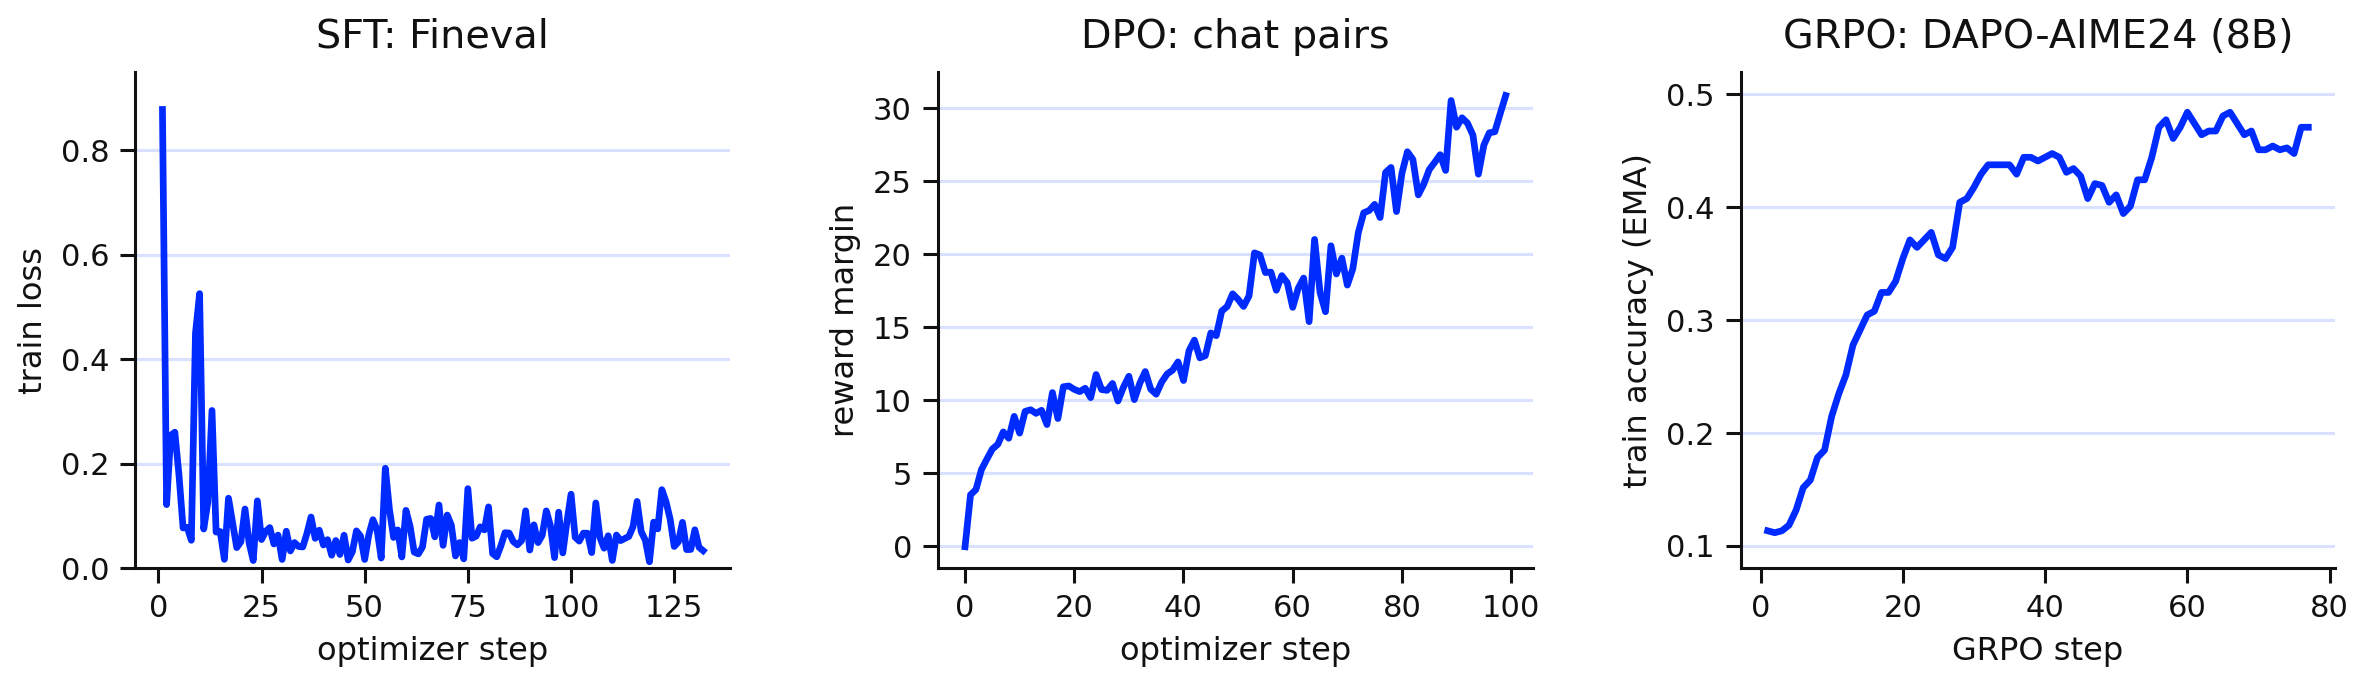
\includegraphics[width=\textwidth]{figures/eval_dense_curves.png}
    \caption{Dense-model learning traces. Each panel keeps the native metric for its training paradigm instead of forcing SFT loss, DPO reward margin, and GRPO train accuracy onto one axis.}
    \label{fig:e3_dense_curves}
\end{figure}

\subsection{Scale Up Across Training Paradigms and Model Scales}
\label{sec:e3_curves}

Dense-model experiments use Qwen3-4B for SFT and DPO, and Qwen3-8B base for GRPO. The SFT rows use FinEval and finance-sentiment benchmarks from the FinGPT evaluation suite~\citep{fineval2023,fingpt2023}. The DPO row uses the chat-DPO recipe's reward-margin trace. The GRPO row uses the Qwen3-8B-base DAPO-AIME24 trace on the 2024 American Invitational Mathematics Examination~\citep{maa_aime2024}. \Cref{fig:e3_dense_curves} shows the learning traces, while \cref{tab:e3_dense_results} separates curve-backed rows from held-out confirmation rows.

Each paradigm exercises a different part of the same lifecycle. SFT tests whether a supervised dataset moves into the adapter, trains through the LoRA path, and produces held-out gains comparable to a full fine-tune; the five FinGPT-suite rows cover finance-domain accuracy and the broader FinEval task at the same time. DPO tests whether a preference-pair objective drives the same adapter through the chat-DPO recipe and increases the chosen-minus-rejected reward margin during optimization. GRPO tests whether a rollout-based RL recipe updates the adapter from on-policy AIME 2024 rollouts. Together, the rows show one adapter type and one export format carrying SFT loss, DPO reward margin, and GRPO train accuracy without any per-paradigm tooling change. \Cref{tab:e3_dense_results} reports the endpoint rows that quantify each of these checks.

\begin{table}[H]
\centering
\scriptsize
\setlength{\tabcolsep}{3.2pt}
\renewcommand{\arraystretch}{1.10}
\caption{Dense-model result rows. The table keeps the native metric for each objective and separates plotted traces from held-out confirmation scores. FPB, FiQA-SA, TFNS, and NWGI are finance-sentiment held-out sets from the FinGPT evaluation suite~\citep{fingpt2023}.}
\label{tab:e3_dense_results}
\fittowidth{%
\begin{tabular}{@{}M{0.14\textwidth}M{0.25\textwidth}M{0.16\textwidth}M{0.17\textwidth}M{0.20\textwidth}@{}}
\toprule
\apphead Paradigm & Benchmark & Metric & Evidence & Result \\
\midrule
\appgroup{5}{SFT: finance suite}
\appkey{SFT} & Fineval & accuracy & held-out score & 0.4226 $\rightarrow$ 0.7811 \\
\appkey{SFT} & FPB & accuracy & held-out score & 0.6906 $\rightarrow$ 0.8804 \\
\appkey{SFT} & FiQA-SA & accuracy & held-out score & 0.8255 $\rightarrow$ 0.8473 \\
\appkey{SFT} & TFNS & accuracy & held-out score & 0.5959 $\rightarrow$ 0.9095 \\
\appkey{SFT} & NWGI & accuracy & held-out score & 0.4954 $\rightarrow$ 0.5925 \\
\appgroup{5}{Preference optimization}
\appkey{DPO} & chat pairs & reward margin & trace endpoint & $-0.03 \rightarrow 30.88$ \\
\appgroup{5}{Reinforcement learning}
\appkey{GRPO} & AIME24 & train accuracy (EMA) & Qwen3-8B trace & $0.11 \rightarrow 0.47$; best raw 0.568 at step 76 \\
\bottomrule
\end{tabular}%
}
\end{table}

The dense rows separate two kinds of evidence under the same adapter lifecycle. The five SFT rows from the FinGPT evaluation suite all confirm large held-out gains over the base Qwen3-4B score: roughly $+36$ points on FinEval, $+19$ on FPB, $+31$ on TFNS, and smaller but consistent moves on FiQA-SA and NWGI. The DPO row reports the reward-margin endpoint from the chat-DPO optimization trace. The GRPO row reports the Qwen3-8B-base DAPO-AIME24 training trace, whose EMA train accuracy rises from 0.11 to 0.47 and whose raw best point reaches 0.568 at step 76. The combined message is paradigm-agnostic: the same lifecycle carries supervised, preference-based, and rollout-based updates without any per-paradigm checkpoint surgery.

MoE experiments add two conditions beyond the dense rows. First, expert routes must be replayed during training-time scoring so that tokens are scored under the MoE path that generated them. Second, large MoE models test whether the adapter/base split survives distributed placement across tensor-parallel and expert-parallel workers. The Qwen3-235B-A22B run uses the Hopper-class \texttt{mint-prod-aliyun} profile: a 32-GPU Megatron trainer with TP=4 and EP=8 (PP=1), paired with a 16-GPU TP=16 serving deployment. The Kimi K2 1.04T countdown-task run uses a 64-GPU H800 deployment with the same LoRA RL path on 32.6B active parameters. \Cref{fig:e3_moe_curves} shows the 30B and 235B AIME24 curves together with the Kimi K2 1T countdown-task RL curve~\citep{liu2025Build}.

\begin{figure}[H]
    \centering
    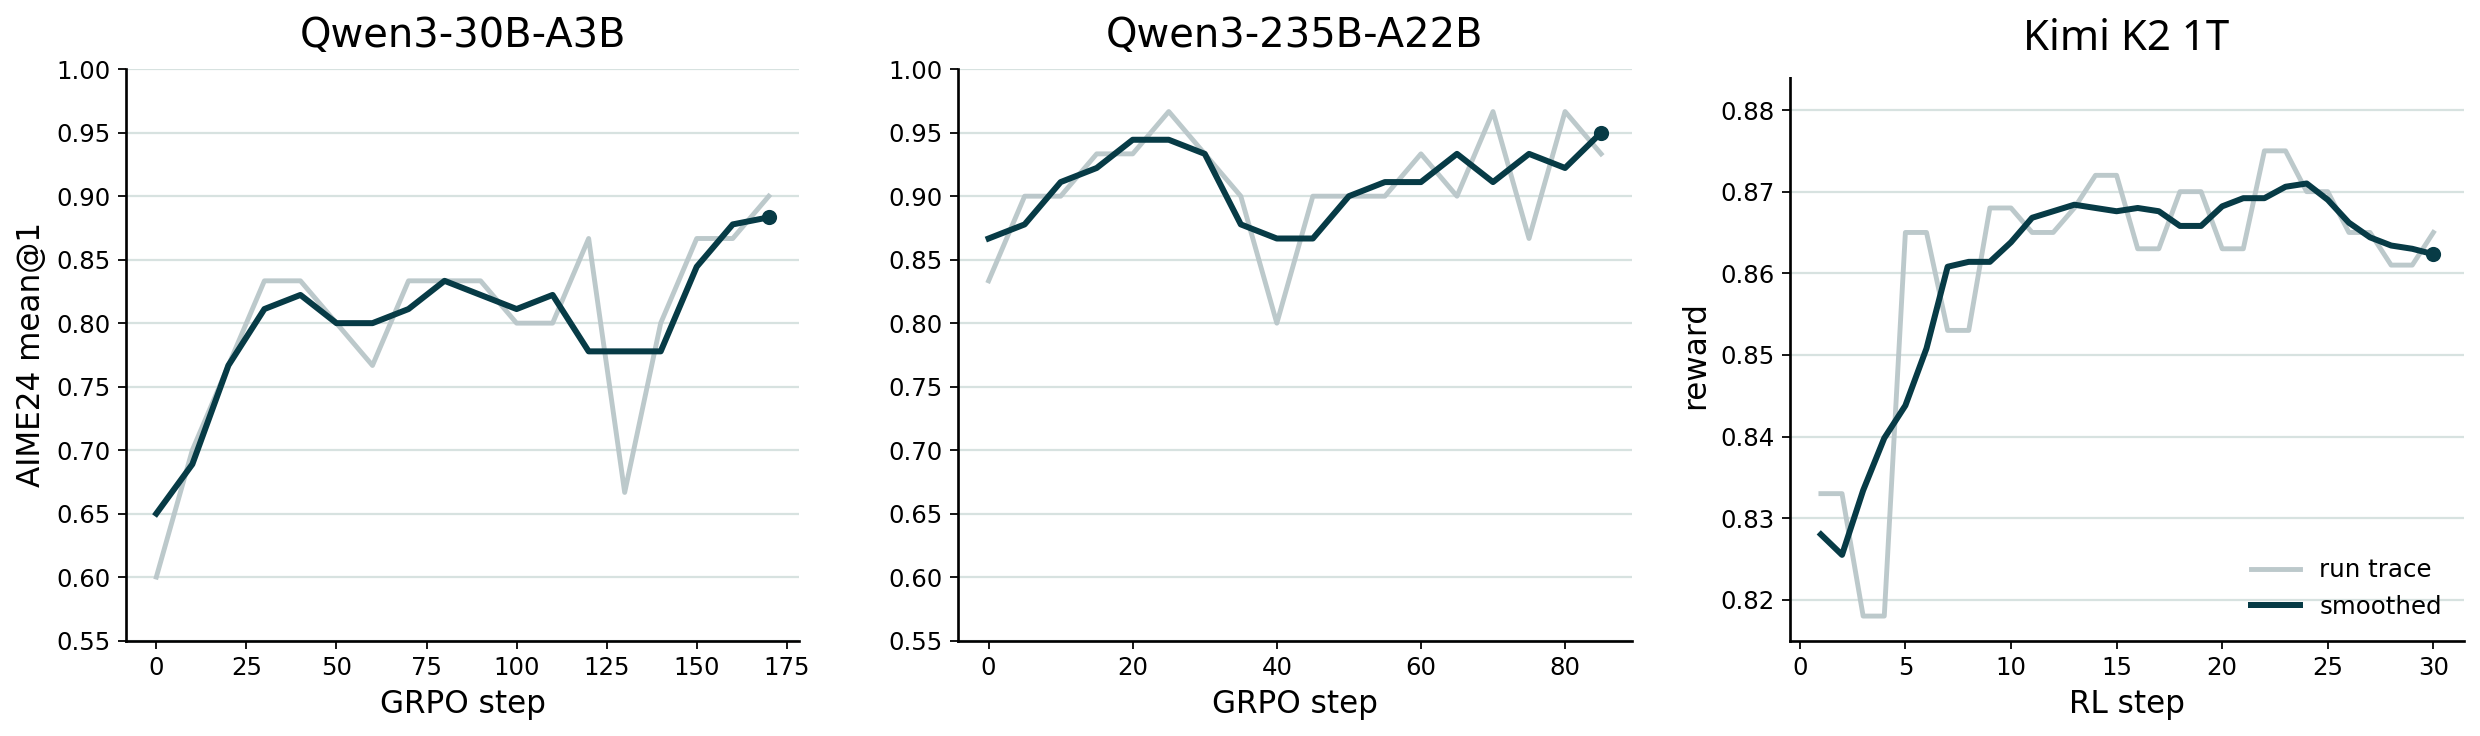
\includegraphics[width=0.98\textwidth]{figures/eval_moe_scale_curves.png}
    \caption{MoE RL curves. The 30B/235B panels use AIME24 mean@1 with aligned y axes and smoothed overlays. The Kimi K2 panel gives the end-to-end LoRA RL reward curve for the 1T countdown-task run~\citep{liu2025Build}.}
    \vspace{-10pt}
    \label{fig:e3_moe_curves}
\end{figure}

The 30B-A3B and 235B-A22B panels share the same y axis to make the scale jump readable. The 30B-A3B AIME24 curve rises from a noisy near-zero start to a stable mid-band by the end of the logged window, while the 235B-A22B curve reaches 0.967 peak mean@1 -- close to saturation on AIME24 under the same LoRA RL path. The Kimi K2 panel switches to task reward instead of an AIME-style accuracy because the countdown task has a different correctness target, but the curve follows the same rollout-update-export-evaluate loop on a 1.04T-parameter base. Together, the three panels close the scale-up claim along the adapter lifecycle: the LoRA adapter remains the policy object across a 30B sparse base, a 235B-A22B Hopper deployment, and a trillion-parameter MoE, with no change to the training-serving handoff between them.

\begin{figure}[H]
    \centering
    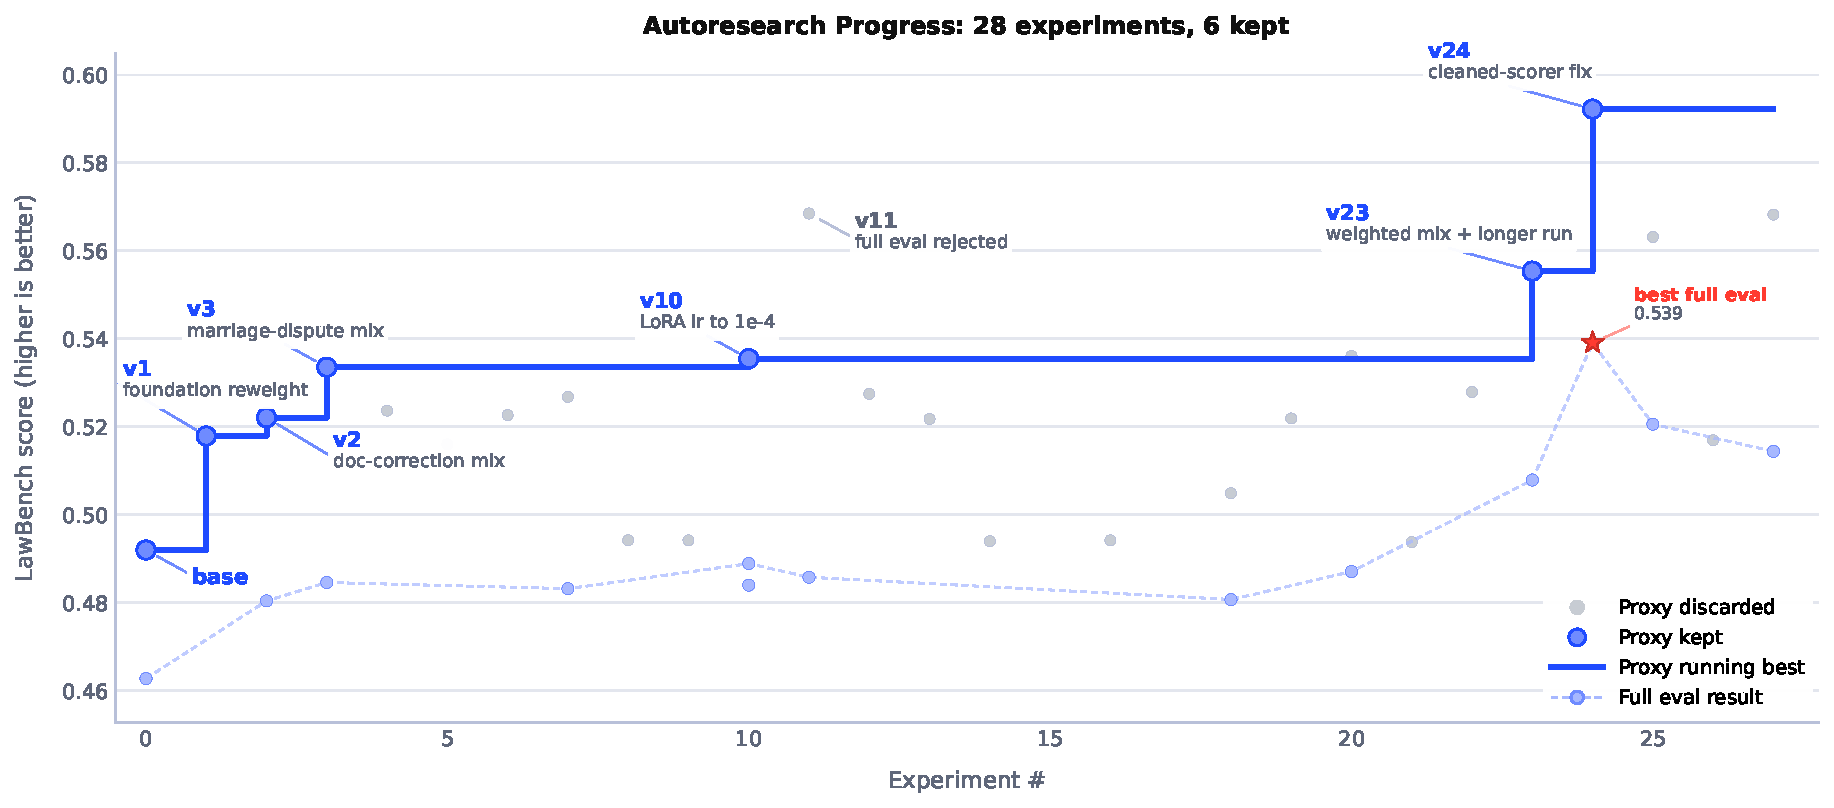
\includegraphics[width=\textwidth]{figures/lawbench_qwen3_4b_autoresearch.pdf}
    \caption{LawBench AutoResearch trace from the cookbook utilities. Pale gray points are proxy-screened candidates that were not promoted, blue-outlined points are kept proxy candidates, the blue step line is the running best among kept candidates, violet points are full LawBench evaluations, and the black diamond is the full-manifest control. The labeled v11 proxy high was rejected after full-benchmark confirmation.}
    \label{fig:e3_autoresearch_lawbench}
\end{figure}


The MoE route counters report how often token-level scoring attempts needed route-consistency handling. On Qwen3-30B, the run with R3 has a mean out-of-route scoring ratio of 0.0013\% across 87 logged steps, while the comparable no-R3 run averages 0.0097\% across 50 logged steps. On Qwen3-235B, the R3 run averages 0.0253\% across 88 logged steps. These counters are small because they are token-level rates, yet they identify the exact failure channel that R3 controls: a token sampled under one expert route should not be scored as if a different route had produced it. The Qwen3-235B curve reaches 0.967 peak mean@1 on AIME24.

AutoResearch evaluates recipe candidates in two stages. Proxy LawBench tasks screen many data-manifest and recipe variants, and selected variants then receive full LawBench confirmation before being counted as improved recipes~\citep{lawbench2024}. FinGPT, DAPO-AIME, and chat-DPO supply confirmed SFT, GRPO, and DPO rows above. The cookbook provides AutoResearch utilities for coding agents to launch MinT runs, screen candidate recipes on proxy LawBench tasks, and promote selected candidates to full LawBench confirmation. In the LawBench run, the base Qwen3-4B full score is 0.4628. The v10 recipe is the earlier learning-rate-tuned line. The high-proxy v11 candidate remains discarded because its full LawBench score is 0.4858, below v10's 0.4889. The full-manifest control reruns the later data manifest without the promoted changes and reaches 0.4712. The maintained v23 weighted-aligned recipe extends the aligned-data line to a fairer exposure budget; it reaches 0.5554 on the proxy screen at step 100 and 0.5079 on the full benchmark~\citep{mint_cookbook2026}. \Cref{fig:e3_autoresearch_lawbench} plots the proxy-search trajectory and full-benchmark confirmation points.

The proxy-versus-full divergence is the methodological signal the cookbook is built around. The v11 candidate set a new proxy high but its full LawBench score fell below v10's; this is the exact failure mode an unsupervised proxy can produce when its task distribution diverges from the full benchmark's. The full-manifest control at 0.4712 shows that the later data manifest alone does not produce the gain, which separates data effects from recipe effects in the same trace. The maintained v23 weighted-aligned line is the candidate that survives both stages, with a proxy reading of 0.5554 at step 100 and a full reading of 0.5079, well above the base 0.4628 and the v10/v11 cluster. Reading the running-best line together with the kept-candidate filter is how AutoResearch decides to record progress instead of celebrating a single high point, and it is the same lifecycle pattern the previous paradigms use: train an adapter, freeze it as a revision, evaluate that exact revision, then decide whether it enters the maintained recipe set.

\FloatBarrier

\begin{table}[H]
\centering
\scriptsize
\setlength{\tabcolsep}{3.2pt}
\renewcommand{\arraystretch}{1.10}
\caption{Policy-population serving bounds on one Qwen3-30B rank-1 serving actor with TP=4.}
\label{tab:e4_serving_summary}
\fittowidth{%
\begin{tabular}{@{}M{0.20\textwidth}M{0.25\textwidth}M{0.25\textwidth}M{0.23\textwidth}@{}}
\toprule
\apphead Resource tier & Question & Measured bound & Takeaway \\
\midrule
\appgroup{4}{Control-plane addressability}
\appkey{Addressable catalog}
& How many policy revisions can requests select from?
& Catalog sweep from 1k to 100k adapters
& Catalog size stays a name-resolution scale; local cache state determines warm/cold latency. \\
\addlinespace

\appgroup{4}{Local adapter cache}
\appkey{CPU adapter cache}
& How many adapters can one actor keep resident?
& 369 loaded adapters at a 512-adapter hotset; 550 loaded adapters under 2048-adapter weak-locality pressure
& CPU memory holds hundreds of adapters; weak locality raises tail latency. \\
\addlinespace

\appkey{Adapters in one GPU batch}
& How many adapters can decoding use?
& 64 distinct adapters in the tested same-batch window
& Batch execution has the smallest measured adapter-diversity window. \\
\addlinespace

\appgroup{4}{Cold-load path}
\appkey{Cold loading}
& What happens on cache misses?
& Warm $N=64$ p95 21.35 s; cold-cache p95 199.81 s; $N=16$ cold-load staircase 1.375--23.267 s
& Different missing adapters are loaded one at a time before decoding. \\
\addlinespace

\appkey{Adapter representation}
& How costly is tensor fanout?
& 37{,}248 tensors to 672 tensors; 1.05$\times$ byte change; 8.5--8.7$\times$ faster live load
& Packing speeds the cache-miss load path by removing small-object fanout. \\
\bottomrule
\end{tabular}%
}
\end{table}

\subsection{Policy-Population Serving}
\label{sec:e4_serving}

Multi-LoRA serving becomes a policy-population problem when many exported adapter revisions are deployable at once. Training still exports a LoRA adapter instead of a full checkpoint, and serving still keeps the base model resident. A request names one policy revision; the serving actor either finds the adapter in the GPU batch, promotes it from the CPU cache, or loads it from shared storage after a cache miss. Only the policies selected by the current batch consume GPU-batch adapter slots.

The serving experiments use Qwen3-30B rank-1 MoE LoRA adapters on one 4-GPU tensor-parallel serving actor, with prompt length 1024 and maximum output length 64. The probes cover the path from request name to generation: catalog expansion from 1k to 100k entries, repeated-hotset and unique-adapter traffic, warm and cold latency, the tested same-batch adapter window, CPU-cache growth, cold-load accounting, and packed tensor loading. Appendix~\cref{tab:app_fleet_model} extends these single-engine measurements into a $10^6$-entry addressable-catalog sizing sketch; the main measurements do not imply that $10^6$ adapters are simultaneously resident or active. \Cref{tab:e4_serving_summary} gives the main bounds.

\paragraph{Adapter cache levels.}
MinT treats each exported adapter revision as an addressable policy revision that can move through three cache levels. The durable catalog names policy revisions that can be requested; the CPU cache is local to one serving actor; the GPU batch is the smaller set attached to a decoding step. A cold load moves a policy revision from the durable catalog into the actor before decoding can begin.

Large catalogs split fleet-level routing from engine-local memory. A million accumulated policy revisions is a catalog and routing problem; one engine keeps only a bounded local cache. The main experiments measure warm/cold behavior across independently run catalogs up to 100k adapters, while Appendix~\cref{tab:app_fleet_model} turns the measured single-engine limits into a $10^6$-adapter capacity model under a 2300-distinct-adapter active-wave assumption. Appendix~\cref{tab:app_memory_loader_accounting} gives the byte and memory accounting behind these cache levels: HBM remains dominated by the resident base model, while CPU memory and adapter object shape determine how many policies can be kept cached near one engine.

\paragraph{Cached adapters and batch diversity.}
Local adapter caches absorb locality before requests touch shared storage. Tenant variants, rollback points, personalization branches, and recent evaluation candidates often recur; broad rollout waves and experiment sweeps have much weaker locality. The service has to support both traffic shapes while keeping CPU cache size separate from same-batch execution.

\begin{figure}[H]
    \centering
    \begin{subfigure}[t]{0.48\textwidth}
        \centering
        \resizebox{\linewidth}{!}{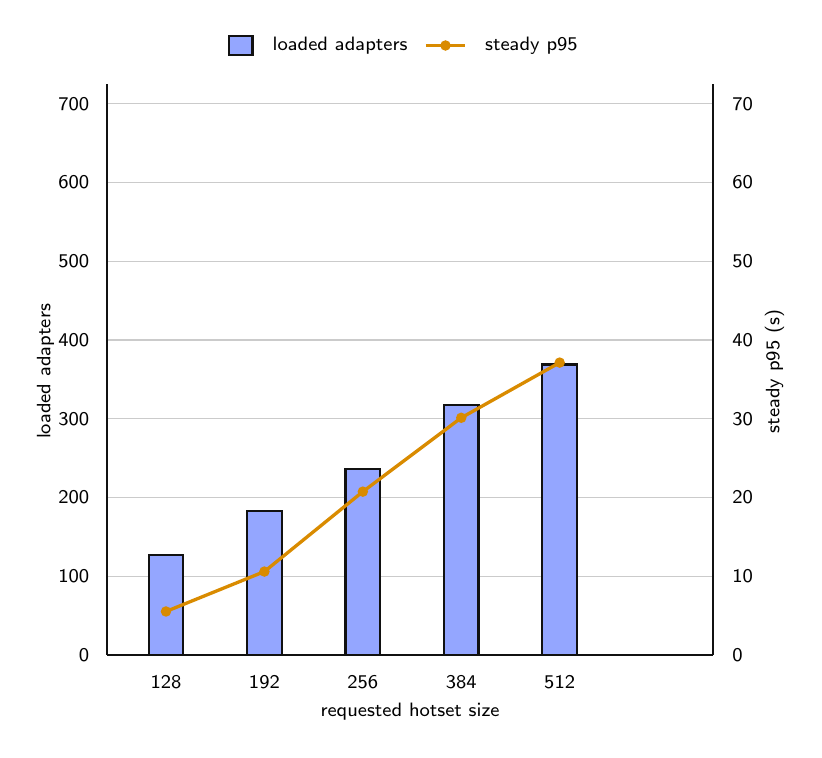
\begin{tikzpicture}[x=1cm,y=1cm,>=stealth,font=\sffamily]
  \definecolor{mintauxamber}{HTML}{D98B00}
  \tikzstyle{axis}=[thick, draw=mindlabfg]
  \tikzstyle{bar}=[fill=mindlabblue!42, draw=mindlabfg, thick]
  \tikzstyle{latency}=[draw=mintauxamber, line width=1.2pt]
  \tikzstyle{label}=[font=\scriptsize\sffamily, align=center]

  \foreach \y/\lval/\rval in {0/0/0,1/100/10,2/200/20,3/300/30,4/400/40,5/500/50,6/600/60,7/700/70} {
    \draw[mindlabfg!22] (0,\y) -- (7.7,\y);
    \node[label, anchor=east] at (-0.10,\y) {\lval};
    \node[label, anchor=west] at (7.82,\y) {\rval};
  }
  \draw[axis] (0,0) -- (0,7.25);
  \draw[axis] (0,0) -- (7.7,0);
  \draw[axis] (7.7,0) -- (7.7,7.25);
  \node[label, rotate=90] at (-0.78,3.6) {loaded adapters};
  \node[label, rotate=90] at (8.48,3.6) {steady p95 (s)};

  \foreach \x/\hot/\loaded/\lat in {
    0.75/128/1.27/0.552,
    2.00/192/1.83/1.059,
    3.25/256/2.36/2.074,
    4.50/384/3.17/3.012,
    5.75/512/3.69/3.713
  } {
    \draw[bar] (\x-0.22,0) rectangle (\x+0.22,\loaded);
    \node[label] at (\x,-0.35) {\hot};
  }

  \draw[latency]
    (0.75,0.552) -- (2.00,1.059) -- (3.25,2.074) --
    (4.50,3.012) -- (5.75,3.713);
  \foreach \x/\y in {0.75/0.552,2.00/1.059,3.25/2.074,4.50/3.012,5.75/3.713} {
    \fill[mintauxamber] (\x,\y) circle (1.9pt);
  }

  \node[label] at (3.85,-0.72) {requested hotset size};
  \draw[bar] (1.55,7.62) rectangle (1.85,7.86);
  \node[label, anchor=west] at (1.98,7.74) {loaded adapters};
  \draw[latency] (4.05,7.74) -- (4.55,7.74);
  \fill[mintauxamber] (4.30,7.74) circle (1.9pt);
  \node[label, anchor=west] at (4.68,7.74) {steady p95};
\end{tikzpicture}
}
        \caption{Repeated-adapter traffic.}
        \label{fig:e4_hotset_ladder}
    \end{subfigure}\hfill
    \begin{subfigure}[t]{0.48\textwidth}
        \centering
        \resizebox{\linewidth}{!}{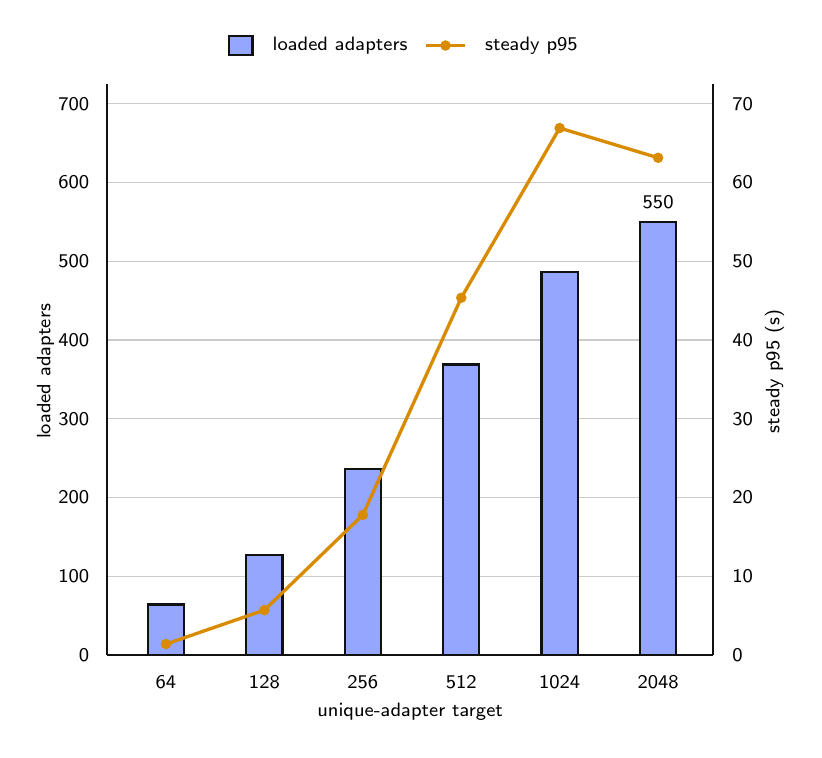
\begin{tikzpicture}[x=1cm,y=1cm,>=stealth,font=\sffamily]
  \definecolor{mintauxamber}{HTML}{D98B00}
  \tikzstyle{axis}=[thick, draw=mindlabfg]
  \tikzstyle{bar}=[fill=mindlabblue!42, draw=mindlabfg, thick]
  \tikzstyle{latency}=[draw=mintauxamber, line width=1.2pt]
  \tikzstyle{label}=[font=\scriptsize\sffamily, align=center]

  \foreach \y/\lval/\rval in {0/0/0,1/100/10,2/200/20,3/300/30,4/400/40,5/500/50,6/600/60,7/700/70} {
    \draw[mindlabfg!22] (0,\y) -- (7.7,\y);
    \node[label, anchor=east] at (-0.10,\y) {\lval};
    \node[label, anchor=west] at (7.82,\y) {\rval};
  }
  \draw[axis] (0,0) -- (0,7.25);
  \draw[axis] (0,0) -- (7.7,0);
  \draw[axis] (7.7,0) -- (7.7,7.25);
  \node[label, rotate=90] at (-0.78,3.6) {loaded adapters};
  \node[label, rotate=90] at (8.48,3.6) {steady p95 (s)};

  \foreach \x/\target/\loaded/\lat in {
    0.75/64/0.64/0.138,
    2.00/128/1.27/0.570,
    3.25/256/2.36/1.779,
    4.50/512/3.69/4.536,
    5.75/1024/4.86/6.692,
    7.00/2048/5.50/6.314
  } {
    \draw[bar] (\x-0.23,0) rectangle (\x+0.23,\loaded);
    \node[label] at (\x,-0.35) {\target};
  }

  \draw[latency]
    (0.75,0.138) -- (2.00,0.570) -- (3.25,1.779) --
    (4.50,4.536) -- (5.75,6.692) -- (7.00,6.314);
  \foreach \x/\y in {0.75/0.138,2.00/0.570,3.25/1.779,4.50/4.536,5.75/6.692,7.00/6.314} {
    \fill[mintauxamber] (\x,\y) circle (1.9pt);
  }
  \node[label, anchor=south] at (7.00,5.55) {550};

  \node[label] at (3.85,-0.72) {unique-adapter target};
  \draw[bar] (1.55,7.62) rectangle (1.85,7.86);
  \node[label, anchor=west] at (1.98,7.74) {loaded adapters};
  \draw[latency] (4.05,7.74) -- (4.55,7.74);
  \fill[mintauxamber] (4.30,7.74) circle (1.9pt);
  \node[label, anchor=west] at (4.68,7.74) {steady p95};
\end{tikzpicture}
}
        \caption{Unique-adapter traffic.}
        \label{fig:e4_true_unique_frontier}
    \end{subfigure}
    \vspace{-10PT}
    \caption{Cached-adapter scaling on one 4-GPU Qwen3-30B rank-1 serving actor. Bars use the left axis for loaded adapters; lines use the right axis for steady p95 latency. The left panel measures locality absorption under repeated-adapter traffic, reaching 369 loaded adapters at a 512-adapter working set. The right panel measures cache growth under weak locality, reaching 550 loaded adapters at a 2048-adapter unique target while p95 rises to 63.14 s.}
    \vspace{-10PT}
    \label{fig:e4_cache_ladders}
\end{figure}

\Cref{fig:e4_cache_ladders} measures these two regimes. Repeated-adapter traffic reaches 369 loaded adapters at a 512-adapter hotset with p95 37.13 s and no errors. Weak-locality traffic reaches 550 loaded adapters at a 2048-adapter unique target with p95 63.14 s and no errors, so it is cache-growth evidence under pressure rather than a clean warm-cache endpoint. Up to target 512 the two panels report essentially the same loaded count (127, 236, and 369), so locality matters only once the request stream exceeds the working set; beyond that, weak-locality p95 saturates rather than diverges, peaking at 66.92 s at target 1024 and settling at 63.14 s at target 2048 as the CPU cache plateaus near 550. Both loaded-adapter counts are larger than the tested same-batch window of 64 distinct adapters: one actor can cache more adapters than it can execute together in one GPU batch. Routing should preserve warm reuse, while batching still has to respect the smaller same-batch adapter limit. Appendix~\cref{tab:app_cache_ladders} gives the ordered ladder data, and Appendix~\cref{tab:app_business_traffic} shows stress probes where long outputs, weak locality, and high concurrency make simple warm-cache assumptions break down.

\paragraph{Cold loading as service work.}
Cold misses expose the cache-miss work inside a policy population. New adapters, rollback points, long-tail personalization branches, and evaluation snapshots keep producing cache misses. A cold miss fetches adapter tensors, builds loader objects, registers the adapter with the serving engine, and only then starts generation. MinT therefore treats cold loading as scheduled service work, with deduplication for repeated cache-miss requests to the same policy and bounded backpressure when too many distinct missing policies arrive together.

\Cref{fig:e4_latency_catalog} shows why this is a separate capacity dimension. CPU-cached requests take the warm regime. Cache-miss requests take the cold regime. Increasing the independently run catalog from 1k to 100k adapters keeps the same warm/cold latency modes; Appendix~\cref{tab:app_path_pool_sweep} reports the full sweep, including one failed cold request in the 100k row. The right panel isolates the controlled cold-miss component: 16 different cache-miss policies form a load staircase from 1.375 s to 23.267 s, about 1.35--1.40 s per policy. Concurrent cache-miss requests for the same missing policy can share one load, while different missing policies remain separate load jobs. Appendix~\cref{tab:app_cold_load_control} decomposes this path into API queueing, shared loads, unique-policy loading, and retryable load rejection.

\begin{figure}[H]
    \centering
    \resizebox{0.92\textwidth}{!}{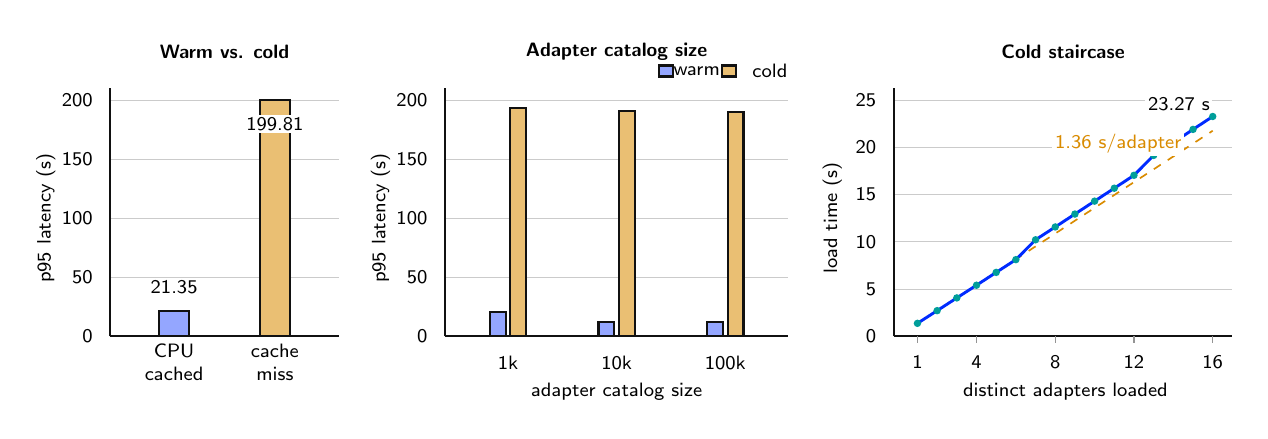
\begin{tikzpicture}[x=1cm,y=1cm,>=stealth,font=\sffamily]
  \definecolor{mintauxteal}{HTML}{009E9A}
  \definecolor{mintauxamber}{HTML}{D98B00}
  \tikzstyle{axis}=[thick, draw=mindlabfg]
  \tikzstyle{warmbar}=[fill=mindlabblue!42, draw=mindlabfg, thick]
  \tikzstyle{coldbar}=[fill=mintauxamber!55, draw=mindlabfg, thick]
  \tikzstyle{observed}=[draw=mindlabblue, line width=1.05pt]
  \tikzstyle{refline}=[draw=mintauxamber, dashed, semithick]
  \tikzstyle{label}=[font=\scriptsize\sffamily, align=center]

  \path[use as bounding box] (-1.05,-0.95) rectangle (14.35,3.92);

  % Panel A: warm versus cache-miss cold latency.
  \begin{scope}[shift={(0,0)}]
    \foreach \y/\lab in {0/0,0.75/50,1.50/100,2.25/150,3.00/200} {
      \draw[mindlabfg!22] (0,\y) -- (2.90,\y);
      \node[label, anchor=east] at (-0.10,\y) {\lab};
    }
    \draw[axis] (0,0) -- (2.90,0);
    \draw[axis] (0,0) -- (0,3.16);
    \node[label, rotate=90] at (-0.82,1.50) {p95 latency (s)};
    \node[label] at (1.45,3.62) {\textbf{Warm vs. cold}};

    \draw[warmbar] (0.62,0) rectangle (1.00,0.320);
    \draw[coldbar] (1.90,0) rectangle (2.28,2.997);
    \node[label] at (0.81,-0.33) {CPU\\cached};
    \node[label] at (2.09,-0.33) {cache\\miss};
    \node[label, anchor=south] at (0.81,0.42) {21.35};
    \node[label, fill=white, inner sep=1pt] at (2.09,2.70) {199.81};
  \end{scope}

  % Panel B: adapter catalog scaling. Same y scale as Panel A.
  \begin{scope}[shift={(4.25,0)}]
    \foreach \y/\lab in {0/0,0.75/50,1.50/100,2.25/150,3.00/200} {
      \draw[mindlabfg!22] (0,\y) -- (4.35,\y);
      \node[label, anchor=east] at (-0.10,\y) {\lab};
    }
    \draw[axis] (0,0) -- (4.35,0);
    \draw[axis] (0,0) -- (0,3.16);
    \node[label, rotate=90] at (-0.82,1.50) {p95 latency (s)};
    \node[label] at (2.18,3.62) {\textbf{Adapter catalog size}};
    \draw[warmbar] (2.72,3.30) rectangle (2.90,3.44);
    \node[label, anchor=west] at (2.78,3.37) {warm};
    \draw[coldbar] (3.52,3.30) rectangle (3.70,3.44);
    \node[label, anchor=west] at (3.78,3.37) {cold};

    \foreach \x/\pool/\warmheight/\coldheight/\warmval/\coldval in {
      0.80/1k/0.313/2.896/20.9/193.0,
      2.18/10k/0.182/2.861/12.2/190.7,
      3.56/100k/0.182/2.846/12.1/189.7
    } {
      \draw[warmbar] (\x-0.23,0) rectangle (\x-0.03,\warmheight);
      \draw[coldbar] (\x+0.03,0) rectangle (\x+0.23,\coldheight);
      \node[label] at (\x,-0.33) {\pool};
    }
    \node[label] at (2.18,-0.70) {adapter catalog size};
  \end{scope}

  % Panel C: cold-load staircase. Same x-axis baseline as Panels A/B.
  \begin{scope}[shift={(9.95,0)}]
    \foreach \y/\lab in {0/0,0.60/5,1.20/10,1.80/15,2.40/20,3.00/25} {
      \draw[mindlabfg!22] (0,\y) -- (4.30,\y);
      \node[label, anchor=east] at (-0.10,\y) {\lab};
    }
    \draw[axis] (0,0) -- (4.30,0);
    \draw[axis] (0,0) -- (0,3.16);
    \node[label, rotate=90] at (-0.78,1.50) {load time (s)};
    \node[label] at (2.15,3.62) {\textbf{Cold staircase}};

    \foreach \x/\lab in {0.30/1,1.05/4,2.05/8,3.05/12,4.05/16} {
      \draw[mindlabfg!45] (\x,0) -- (\x,-0.08);
      \node[label] at (\x,-0.33) {\lab};
    }
    \node[label] at (2.18,-0.70) {distinct adapters loaded};

    \draw[refline] (0.30,0.163) -- (4.05,2.611);
    \draw[observed]
      (0.30,0.165) -- (0.55,0.326) -- (0.80,0.488) -- (1.05,0.649)
      -- (1.30,0.812) -- (1.55,0.974) -- (1.80,1.226) -- (2.05,1.389)
      -- (2.30,1.553) -- (2.55,1.717) -- (2.80,1.881) -- (3.05,2.045)
      -- (3.30,2.298) -- (3.55,2.461) -- (3.80,2.628) -- (4.05,2.792);
    \foreach \x/\y in {
      0.30/0.165,0.55/0.326,0.80/0.488,1.05/0.649,
      1.30/0.812,1.55/0.974,1.80/1.226,2.05/1.389,
      2.30/1.553,2.55/1.717,2.80/1.881,3.05/2.045,
      3.30/2.298,3.55/2.461,3.80/2.628,4.05/2.792
    } {
      \fill[mintauxteal] (\x,\y) circle (1.35pt);
    }
    \node[label, text=mintauxamber, fill=white, inner sep=1pt] at (2.85,2.45) {1.36 s/adapter};
    \node[label, fill=white, inner sep=1pt] at (3.62,2.95) {23.27 s};
  \end{scope}
\end{tikzpicture}
}
    \vspace{-10PT}
    \caption{Warm routing and bounded cold-load cost. Left: CPU-cached adapters take the warm latency path, while cache-miss policies take the cold path. Middle: warm measurements stay in the warm p95-latency regime and cold measurements stay in the cold p95-latency regime as independently run adapter catalogs grow to 100k entries. Right: 16 different cache-miss policies form a serialized load staircase from 1.375 s to 23.267 s, about 1.35--1.40 s per policy.}
    \vspace{-10PT}
    \label{fig:e4_latency_catalog}
\end{figure}

\paragraph{Cold-load representation.}
The load staircase also explains why the adapter file format matters. A rank-1 MoE LoRA adapter is moderate in bytes, while the measured adapter file is fragmented into 37{,}248 tensor objects, mostly tiny expert tensors. In these probes, local-disk staging shortened the read path; it left tensor fanout, Python object creation, and loader-side registration work unchanged. MinT therefore packs MoE expert tensors into a serving representation with nearly unchanged declared bytes, reducing object fanout before the engine loads the policy.

\begin{table}[H]
\centering
\scriptsize
\setlength{\tabcolsep}{4.0pt}
\renewcommand{\arraystretch}{1.08}
\caption{Packed MoE LoRA loading reduces cold-load overhead by removing tensor fanout. The byte-size change is small; the speedup comes from replacing many tiny tensor objects with a compact serving representation. The final three rows report the median duration of one live load call measured at each cache-miss burst size.}
\label{tab:e4_packed_loader}
\fittowidth{%
\begin{tabular}{@{}M{0.32\textwidth}M{0.16\textwidth}M{0.16\textwidth}M{0.24\textwidth}@{}}
\toprule
\apphead Metric & Original & Packed & Effect \\
\midrule
\appgroup{4}{Adapter-file shape}
\appkey{File size} & 110.75 MB & 105.58 MB & 1.05$\times$ smaller \\
\appkey{Tensor objects} & 37{,}248 & 672 & 55.4$\times$ fewer \\
\appgroup{4}{Cold-load slice}
\appkey{Read tensors} & 0.3669 s & 0.0067 s & 54.8$\times$ faster \\
\appkey{Build loader objects} & 0.7540 s & 0.0256 s & 29.5$\times$ faster \\
\appgroup{4}{Live engine loading}
\appkey{$N=4$ live load} & 1.363 s & 0.156 s & 8.7$\times$ faster \\
\appkey{$N=8$ live load} & 1.361 s & 0.159 s & 8.6$\times$ faster \\
\appkey{$N=16$ live load} & 1.388 s & 0.164 s & 8.5$\times$ faster \\
\bottomrule
\end{tabular}%
}
\end{table}

\Cref{tab:e4_packed_loader} shows the effect. Packing changes file size only from 110.75 MB to 105.58 MB and reduces tensor objects from 37{,}248 to 672. The direct loader slice improves by 29.5--54.8$\times$, and live engine loading for $N=4$, $N=8$, and $N=16$ improves by 8.5--8.7$\times$, with packed live-load medians under 0.2 seconds. This number refers to the live engine-load slice after packing; end-to-end cold latency still includes routing, queueing, fetch, and generation. The measured speedup comes from object layout: the serving representation removes the small-object storm on cache misses while the declared tensor bytes stay nearly unchanged.

\FloatBarrier
Together, these measurements locate the serving work for policy populations. Catalog lookup and raw LoRA count are control-plane scales in the measured sweep; CPU-cache size, tested same-batch diversity, and unique cold-load cost are online execution scales. Routing and prewarming turn recurring traffic into CPU-cache hits. Batch construction respects the smaller same-batch adapter limit. Cache misses enter an explicit cold-load stage before sampling latency begins. Packing reduces the load staircase itself, making cache misses cheaper without changing the base-model deployment or the addressable policy revision. Appendix~\cref{app:serving} contains the full ladders, accounting tables, stress probes, and fleet-level sizing sketch behind this contract.
\FloatBarrier

\section{Related Work}
\label{sec:related}

\paragraph{Post-training workload.}
MinT targets a workload where post-training leaves many policy variants over a smaller set of base models. Yao argues that future progress shifts more weight toward problem definition, evaluation, and agent-environment interaction~\citep{yao_second_half_2025}. Silver and Sutton frame future agents as learning from streams of experience in addition to static human data~\citep{silver_sutton_experience_2025}. Recent frontier-model reports expose the same systems pressure through reasoning, coding, tool use, executable environments, asynchronous agent RL, and long-horizon evaluation~\citep{deepseek_v4_release_2026,deepseekv4_2026,glm5_2026,kimi_k25_2026,minimax_m27_2026,qwen35_2026,openai_gpt55_2026,anthropic_opus45_2025,anthropic_agent_autonomy_2026}. These workloads produce task variants, evaluation candidates, product branches, tenant adapters, rollback points, and personal adapters that share base models while retaining separate histories.

\paragraph{Service interfaces.}
Remote post-training interfaces make training loops programmable. Tinker exposes low-level post-training primitives through a remote service~\citep{tinker2025,tinker_cookbook}. SkyRL tx implements a Tinker-style backend and documents model and benchmark coverage across Qwen3 dense and MoE models, Llama 3, DeepSeek V3, GSM8K, and DAPO/AIME recipes~\citep{skyrl_tx}. OpenTinker frames a broader RL-as-a-Service stack around agents, environments, protocols, scheduling, training, and inference~\citep{opentinker2026}. Tinker specifies how users program remote post-training; MinT keeps a compatible programming surface and defines the LoRA-specific service path underneath it: policy record, training checkpoint, rollout record, exported adapter revision, and adapter cache state.

\paragraph{RL execution systems.}
HybridFlow/verl, AReaL, OpenRLHF, Relax, ROLL, StreamRL, AsyncFlow, Laminar, and NeMo-Aligner study rollout scheduling, colocated and disaggregated execution, asynchronous optimization, GPU utilization, failure isolation, and end-task quality~\citep{hybridflow2025,areal2025,openrlhf2024,relax2026,roll2025,streamrl2025,asyncflow2025,laminar2025,nemoaligner2024}. Their central systems objects are actors, rollout replicas, parameter services, queues, and placement groups. MinT uses the same execution concerns and adds LoRA-specific service state: adapter revisions, optimizer state, rollout records, MoE route records, DSA correction metadata, exported adapters, and adapter cache state stay tied to the policy that produced them.

\paragraph{Training-serving consistency.}
Modern RL pipelines often generate rollouts through an inference engine and score them through a training backend. Yao et al. study token-probability gaps in hybrid vLLM/FSDP pipelines and propose truncated importance sampling~\citep{rollout_training_mismatch2025}. Jet-RL shows that mixed BF16 training and FP8 rollout can destabilize on-policy RL under long generations, then uses a unified precision flow to reduce numerical mismatch~\citep{jetrl2026}. R3 studies MoE router disagreement between training and inference and reuses inference-time expert-route records during training~\citep{r3_moe_router2025}. MinT addresses the same problem by storing the adapter revision, rollout record, MoE route or DSA correction metadata, and served evaluation path that name which behavior generated and scored a token.

\paragraph{Parameter-efficient tuning and multi-LoRA training.}
LoRA freezes the base model and trains low-rank matrices attached to selected layers~\citep{lora2022}. AdaLoRA allocates rank budget across matrices according to importance~\citep{adalora2023}. QLoRA combines frozen quantized bases with LoRA updates for memory-efficient fine-tuning~\citep{qlora2023}. LoRA Without Regret argues that LoRA can reach strong post-training quality~\citep{lora_without_regret_2025}, supporting the premise that LoRA can be more than a memory-saving approximation. MinT turns that premise into managed infrastructure for RL service operation: each update restores one adapter and optimizer state over a resident base, each export produces a serving revision, and each rollout or serving request selects that revision through cache and residency state.

\paragraph{Multi-LoRA serving.}
Multi-LoRA serving systems optimize inference after adapters already exist. Punica, S-LoRA, dLoRA, dynamic operator optimization, and vLLM improve batching, memory management, scheduling, and kernels for many adapters over a shared base~\citep{punica2024,slora2023,dlora2024,zhou2025dynamic,vllm2023}. Compress then Serve reduces adapter storage and serving overhead through individual and joint LoRA compression~\citep{compress_then_serve2024}. FastLibra manages LoRA and KV cache dependencies in a unified HBM cache~\citep{fastlibra2025}. LoRAServe handles rank heterogeneity, placement, and routing across distributed LoRA serving clusters~\citep{loraserve2025}. MinT connects the serving catalog to the training lifecycle: an addressable adapter is an exported revision of a trained policy, and a cache miss reloads that revision from the policy's exported adapter file.

\paragraph{Large-model infrastructure.}
Ray provides the distributed execution framework used by many AI systems~\citep{ray2018}. Megatron-LM, Efficient Megatron-LM, ZeRO, and MoE Parallel Folding provide the model-parallel, memory-partitioning, and MoE-parallel techniques that make large-model and sparse-MoE training practical~\citep{megatronlm2019,efficient_megatronlm2021,zero2019,moe_parallel_folding2026}. DeepSeek-V4 describes large-model infrastructure through concrete state units such as hybrid KV cache entries, state caches, on-disk cache storage, rollout WALs, and teacher-state scheduling~\citep{deepseekv4_2026}. MinT applies the same resource-accounting style to LoRA RL: base deployments stay resident, adapter revisions move across subsystems, and adapter cache state controls which exported policies are hot.

\section{Conclusion}

Post-training now couples rollout, update, evaluation, serving, scheduling, and data movement around many policy variants over a small number of expensive base-model deployments. Full-checkpoint workflows make every task branch, benchmark candidate, product version, tenant variant, rollback point, or personal policy look like another complete model deployment. This abstraction does not scale when the target workload is a large and continuously changing population of trained behaviors over shared frontier bases.

MinT makes exported LoRA adapter revisions the managed unit for this setting. Base-model deployments remain resident, while adapter revisions carry trained behavior through rollout, update, export, evaluation, serving, and rollback. The adapter revision is the behavior-carrying payload; the policy record is the service state that makes that payload reproducible, schedulable, and durable across worker changes, training checkpoints, rollout records, and serving-cache movement.

The measurements validate the same adapter-revision path along three scaling axes. \textit{Scale Up} supports LoRA RL on dense and MoE architectures with model-parallel training and serving paths exercised beyond 1T total parameters. \textit{Scale Down} removes full-checkpoint materialization from the training-serving handoff: adapter-only handoff reduces the measured handoff step by $18.3\times$ on a 4B dense model and by $2.85\times$ on a 30B MoE model, while concurrent multi-policy GRPO shortens wall time by $1.77\times$ and $1.45\times$ under the same resident-base allocation. \textit{Scale Out} separates durable policy addressability from CPU/GPU hot working sets: the serving path supports $10^6$-scale addressable policy catalogs, with measured single-engine sweeps through 100K entries and thousand-adapter active waves at cluster scale; first-touch cold loading becomes scheduled service work, and packed MoE LoRA tensors improve live engine loading by $8.5$--$8.7\times$.

Together, these results show that multi-tenant LoRA training services can be made practical without turning every trained policy into a full-model server. MinT lets policy count grow through adapter revisions, policy records, cache tiers, and controlled cold-load admission, while selected revisions train and serve over bounded resident working sets. This makes LoRA a service-level unit for large-scale post-training today and a practical path toward larger populations of organizational and personal policies over shared 1T-class base models.

\bibliographystyle{plainnat}
\bibliography{paper}

\newpage
\begin{appendices}
\section{Author List}
\label{app:author_list}

Names are listed alphabetically.

\paragraph{Core Contributors.}
\begin{sloppypar}
Andrew Chen, Cleon Cheng, Steven Chiang, Nolan Ho, Andrew Lei, Lucian Li, Kieran Liu, Irvine Lu, Pony Ma, Rio Yang, Di Zhang, Adrian Zhou.
\end{sloppypar}

\paragraph{Team.}
\begin{sloppypar}
Song Cao, Vic Cao, Kaijie Chen, Bunny Fan, Hera Feng, Huan Feng, Arthur Fu, Jun Gao, Hongquan Gu, Aaron Guan, Mutian Hong, Hailee Hou, Peixuan Hua, Charles Huang, Miles Jiang, Nora Jiang, Yuyi Jiang, Autumn Jin, Fancy Kong, Kyrie Lei, Alexy Li, Dawn Li, Ray Li, Theo Li, Jiayi Lin, Domini Liu, Heshan Liu, Kairus Liu, Logan Liu, Maeve Luo, Runism Lv, Pony Ma, Verity Niu, Anson Qiu, Vincent Wang, Maxwell Yao, Regis Ye, Wenlin Ye, Yanying Ye, Josh Ying, Danney Zeng, Salmon Zhan, Anya Zhang, Ruijia Zhang, Sueky Zhang, Ya Zhang, Wei Zhao, Ada Zhou, Sizer Zhou, Xinyue Zhu, Murphy Zhuang.
\end{sloppypar}

\section{Additional Serving Measurements}
\label{app:serving}

This appendix expands the serving-side measurements used in \cref{sec:e4_serving}. The tables use the same serving quantities as the main text: catalog size, CPU-cached adapters, adapters in one GPU batch, and the cold-load path that loads an adapter when a request selects an entry outside the actor's local cache. The order separates exploratory probes that rule out simple explanations, measurements that identify the serving limit, and follow-up probes that reduce or isolate that limit.

Several rows intentionally leave the clean warm path. They create weak locality, cold churn, long online generations, or high concurrency so that the failure mode is visible rather than hidden inside average latency. We keep them in the appendix because they identify the control points that a MinT deployment must own: routing for warm reuse, prewarming for predictable waves, bounded cold loading for cache-miss traffic, and lower-fanout adapter representation for unavoidable misses. The shaded bands in the tables separate cache levels and probe families, so a reader can scan from the MinT service path to the measured limit without treating every row as the same kind of claim.

\paragraph{Adapter memory and representation.}
\Cref{tab:app_memory_loader_accounting} separates adapter bytes, tensor fanout, CPU cache footprint, and base-model HBM footprint. This accounting explains why the packed loader experiment matters. The measured adapter is moderate in byte size and fragmented into tens of thousands of small tensors, most of them no larger than 4 KB. Cold loading therefore pays object and registration overhead even when the total bytes are small.

\begin{table}[H]
\centering
\scriptsize
\setlength{\tabcolsep}{4pt}
\renewcommand{\arraystretch}{1.08}
\caption{Memory and representation accounting for the measured 30B MoE LoRA adapter files. The rows separate byte size from object fanout and cache pressure.}
\label{tab:app_memory_loader_accounting}
\fittowidth{%
\begin{tabular}{@{}M{0.18\textwidth}M{0.24\textwidth}M{0.27\textwidth}M{0.23\textwidth}@{}}
\toprule
\apphead Tier / object & Item & Measurement & Serving implication \\
\midrule
\appgroup{4}{Adapter-file shape}
Adapter file & Adapter bytes & 110.75 MB file; 105.5 MB declared tensor bytes & Bytes are moderate for a 30B rank-1 adapter. \\
Adapter file & Tensor fanout & 37{,}248 tensors; 37{,}152 no larger than 4 KB & Object fanout dominates cold load work. \\
\appgroup{4}{Resident execution footprint}
CPU warm tier & CPU cache footprint & 586.8 MB/LoRA across 4 TP workers; 146.7 MB/worker & CPU cache is the per-engine cache limit. \\
GPU batch tier & GPU memory & $N=64$ snapshots show about 272 GiB engine HBM footprint & Base deployment dominates HBM pressure. \\
\appgroup{4}{Packed cold-load representation}
Adapter-file format & Packed representation & 37{,}248 $\rightarrow$ 672 tensors; 110.75 $\rightarrow$ 105.58 MB & Packing removes fanout; bytes stay nearly unchanged. \\
\bottomrule
\end{tabular}%
}
\end{table}

\paragraph{Adapter catalog size.}
\Cref{tab:app_path_pool_sweep} varies the adapter catalog from 1k to 100k entries. The warm/cold split persists across the sweep and the measured tail appears when many distinct cold adapters enter cold loading. These rows support the main-text claim that MinT should keep catalog resolution in the control plane and manage cache state and cold loading in the serving plane.

\begin{table}[H]
\centering
\scriptsize
\setlength{\tabcolsep}{4pt}
\renewcommand{\arraystretch}{1.06}
\caption{Adapter catalog sweep for $N=64$ serving. Warm and cold rows are split so the stable regime gap is visible at each catalog size.}
\label{tab:app_path_pool_sweep}
\fittowidth{%
\begin{tabular}{@{}M{0.13\textwidth}M{0.13\textwidth}ccccM{0.27\textwidth}@{}}
\toprule
\apphead Catalog & Regime & Success & Drain & p95 & Distinct & Readout \\
\midrule
1k & \appkey{warm} & 64/64 & 21.16 s & 20.89 s & 51 & catalog lookup stays in the warm regime \\
1k & \appkey{cold} & 64/64 & 193.23 s & 193.04 s & 56 & cold loading dominates \\
\addlinespace
10k & \appkey{warm} & 64/64 & 12.56 s & 12.16 s & 64 & larger catalog stays in the warm mode \\
10k & \appkey{cold} & 64/64 & 190.99 s & 190.73 s & 56 & cold regime persists \\
\addlinespace
100k & \appkey{warm} & 64/64 & 20.35 s & 12.12 s & 63 & 100k-entry catalog remains addressable \\
100k & \appkey{cold} & 63/64 & 190.08 s & 189.73 s & 56 & tail follows cold loading \\
\bottomrule
\end{tabular}%
}
\end{table}

\paragraph{Cached working sets.}
\Cref{tab:app_cache_ladders} gives the ordered data behind the warm-cache claim in \cref{fig:e4_cache_ladders}. The repeated-hotset rows model adapter locality after routing has found a useful engine placement. The unique-adapter rows remove this locality and measure how many distinct adapters can become cached near one engine before the run stops being a clean warm-path claim. These measurements define the CPU-side tier between the durable adapter catalog and the same-batch adapter window.

\begin{table}[H]
\centering
\scriptsize
\setlength{\tabcolsep}{3.4pt}
\renewcommand{\arraystretch}{1.05}
\caption{Cached-working-set ladder on one 4-GPU Qwen3-30B rank-1 serving actor. Shaded group rows separate routed locality from unique-adapter load pressure.}
\label{tab:app_cache_ladders}
\fittowidth{%
\begin{tabular}{@{}M{0.20\textwidth}cccccM{0.22\textwidth}@{}}
\toprule
\apphead Regime & Target & Loaded & Steady p95 & Errors & Tier & Readout \\
\midrule
\appgroup{7}{Routed locality: repeated hotsets}
Repeated hotsets & 128 & 127 & 5.52 s & 0/3200 & CPU warm & baseline warm tier \\
Repeated hotsets & 192 & 183 & 10.59 s & 0/3200 & CPU warm & locality preserved \\
Repeated hotsets & 256 & 236 & 20.74 s & 0/3200 & CPU warm & p95 rises with hotset \\
Repeated hotsets & 384 & 317 & 30.12 s & 0/3200 & CPU warm & larger cached set \\
Repeated hotsets & 512 & 369 & 37.13 s & 0/3200 & CPU warm & endpoint in figure \\
\appgroup{7}{Unique-adapter calibration: clean active-window probes}
Unique adapters & 16 & 16 & 1.22 s & 0 & GPU active & exact target \\
Unique adapters & 32 & 32 & 1.34 s & 0 & GPU active & exact target \\
Unique adapters & 64 & 64 & 1.41 s & 0 & GPU active & same-batch frontier \\
\appgroup{7}{Unique-adapter ladder: pressure on local cache}
Unique adapters & 128 & 127 & 5.70 s & 0 & CPU warm & loading begins \\
Unique adapters & 192 & 183 & 10.57 s & 0 & CPU warm & mirrors hotset count \\
Unique adapters & 256 & 236 & 17.79 s & 0 & CPU warm & cache growth \\
Unique adapters & 384 & 317 & 38.37 s & 0 & CPU warm & tail appears \\
Unique adapters & 512 & 369 & 45.36 s & 0 & CPU warm & warm cache still grows \\
Unique adapters & 640 & 410 & 59.01 s & 0 & CPU warm & diminishing cache growth \\
Unique adapters & 768 & 440 & 62.85 s & 0 & CPU warm & near plateau \\
Unique adapters & 896 & 466 & 64.66 s & 0 & CPU warm & near plateau \\
Unique adapters & 1024 & 486 & 66.92 s & 0 & CPU warm & mid-ladder endpoint \\
\appgroup{7}{Unique-adapter high ladder: cache plateau}
Unique adapters & 1280 & 513 & 60.91 s & 0 & CPU warm & plateau persists \\
Unique adapters & 1536 & 525 & 60.95 s & 0 & CPU warm & slow cache growth \\
Unique adapters & 1792 & 537 & 59.95 s & 0 & CPU warm & stable p95 band \\
Unique adapters & 2048 & 550 & 63.14 s & 0 & CPU warm & largest measured target \\
\bottomrule
\end{tabular}%
}
\end{table}

\paragraph{Mixed online-length stress traffic.}
\Cref{tab:app_business_traffic} intentionally leaves the clean warm-path setting. These rows combine mixed output lengths, high concurrency, weak locality, prewarm changes, and different slot limits to show where simple routing choices stop being enough. The sticky-hash row is a negative probe: fixed hashing alone fails to provide cache-aware routing under this stress shape. The GPU-slots-64 row is a bounded probe; it verifies a slot-limit setting over two rounds, with long-run stability left outside this claim.

\begin{table}[t]
\centering
\scriptsize
\setlength{\tabcolsep}{2.8pt}
\renewcommand{\arraystretch}{1.05}
\caption{Mixed online-length traffic on a 2048-adapter catalog. The GPU/CPU column gives the GPU-batch LoRA slot limit and the CPU-cache LoRA limit.}
\label{tab:app_business_traffic}
\fittowidth{%
\begin{tabular}{@{}M{0.18\textwidth}cM{0.10\textwidth}cM{0.10\textwidth}ccccM{0.16\textwidth}@{}}
\toprule
\apphead Probe & C & GPU/CPU & Prewarm & Success & Err. & p50 & p95 & p99 & Interpretation \\
\midrule
\appgroup{10}{Single-route stress envelope}
Single route & 8 & 32/1024 & 128 & 256/256 & 0.00\% & 28.79 & 66.23 & 70.47 & low-concurrency baseline \\
Single route & 16 & 32/1024 & 128 & 499/512 & 2.54\% & 63.18 & 134.03 & 179.74 & tail begins to rise \\
Single route & 32 & 32/1024 & 128 & 969/1024 & 5.37\% & 124.35 & 320.82 & 358.71 & queueing and churn visible \\
Single route & 128 & 32/1024 & 0 & 4032/4096 & 1.56\% & 508.92 & 1028.08 & 1403.44 & high-concurrency stress \\
Single route & 230 & 32/1024 & 0 & 7037/7360 & 4.39\% & 967.10 & 1469.37 & 1717.43 & no-prewarm reference \\
Single route & 230 & 32/2048 & 164 & 6707/7360 & 8.87\% & 926.94 & 1441.86 & 1710.01 & slots alone leave tail high \\
\appgroup{10}{Routing and slot probes}
Sticky hash, 2 replicas & 230 & 32/2048 & 164 & 3737/7360 & 49.23\% & 925.62 & 1435.62 & 1746.58 & naive fixed hashing unstable \\
GPU slots 64, 2 rounds & 230 & 64/2048 & 164 & 460/460 & 0.00\% & 848.98 & 1351.34 & 1690.24 & bounded slot-limit probe \\
\bottomrule
\end{tabular}%
}
\end{table}

\begin{table}[t]
\centering
\scriptsize
\setlength{\tabcolsep}{3pt}
\renewcommand{\arraystretch}{1.08}
\caption{Cold-load accounting and service protection.}
\label{tab:app_cold_load_control}
\fittowidth{%
\begin{tabular}{@{}M{0.09\textwidth}M{0.22\textwidth}M{0.29\textwidth}M{0.19\textwidth}M{0.17\textwidth}@{}}
\toprule
\apphead ID & Probe & Measured result & Mechanism isolated & Design response \\
\midrule
\appkey{A1} & Same-server no-warm, $N=64$ & Unique-no-warm p95 125.35 s; load median 60.27 s; queue wait median 0.010 s & LoRA loading drives waiting before generation; API queueing is small. & Separate cold loading from sampling latency. \\
\addlinespace
\appkey{A2} & Same adapter vs unique adapters, $N=16$ & Same-adapter load median 1.56 s; unique adapters form 1.47, 2.84, 4.23, $\ldots$, 23.83 s staircase & Repeated cache-miss requests can share one load. & Reduce unique cold misses through routing and prewarming. \\
\addlinespace
\appkey{A3} & Structured add timing, $N=16$ & Engine time median 1.370 s; lock-wait median 10.890 s; total load p95 21.900 s & Exclusive writer/load path serializes unique loads. & Budget unique cold-load capacity per engine. \\
\addlinespace
\appkey{A4} & Bounded cold-load probe & Max in-flight 1 and queue depth 1: a 4-request cold burst loads 2 and rejects 2 & Cold pressure can be observable and retryable. & Prefer bounded backpressure over unbounded blocking. \\
\bottomrule
\end{tabular}%
}
\vspace{-10pt}
\end{table}

\begin{table}[H]
\centering
\scriptsize
\setlength{\tabcolsep}{3.4pt}
\renewcommand{\arraystretch}{1.08}
\caption{Capacity-planning sketch from measured per-engine limits to a 1M-entry accumulated adapter catalog and a 2300-distinct-adapter active-wave stress envelope.}
\label{tab:app_fleet_model}
\fittowidth{%
\begin{tabular}{@{}M{0.22\textwidth}M{0.25\textwidth}ccM{0.23\textwidth}@{}}
\toprule
\apphead Axis & Sizing rule & Engines & GPUs & System interpretation \\
\midrule
\appgroup{5}{Warm-path placement}
Warm distinct concurrency & $\lceil 2300/64 \rceil$ & 36 & 144 & ideal placement by same-batch adapter diversity \\
Warm headroom band & $36\times\{1.2,1.33,1.5\}$ & 44--54 & 176--216 & margin for skew, retries, and imperfect routing \\
Warm throughput floor & 60 s SLO; 2.57 req/s/engine & 15 & 60 & throughput-only floor; ignores distinct placement \\
\appgroup{5}{Cold-path isolation}
Cold-load rate & 38.3 cold LoRA/s; 0.7/engine & 55 & 220 & rates the cold-load service with burst tail tracked separately \\
Cold-burst isolation & 2300 cold uniques; $\le 32$/engine & 72 & 288 & isolates worst-case first touch through prewarm or backpressure \\
\bottomrule
\end{tabular}%
}
\end{table}

\paragraph{Cold-load accounting.}
\Cref{tab:app_cold_load_control} decomposes the cold path into API queueing, shared loads for repeated cache-miss requests, unique-adapter loading, and bounded backpressure. The probes show that the bottleneck is unique cold adapter loading into one engine. Requests wait before generation on LoRA loading; the measured API queue wait is small. Deduplicating identical missing adapters avoids repeated load work, while distinct cold adapters remain separate load jobs. This supports the main-text claim that cold loading is scheduled service work before ordinary sampling latency.

\paragraph{Fleet-level sizing sketch.}
\Cref{tab:app_fleet_model} uses measured single-engine limits as sizing inputs for a larger MinT deployment. This table is a $10^6$-adapter capacity model under a 2300-distinct-adapter active-wave assumption. The main serving experiments sweep adapter catalogs up to 100k entries. The extrapolation asks how many engines would be needed if a larger accumulated adapter catalog produced that active wave before routing or prewarming restored locality. The 60 s service-level objective is the warm-response target used for the throughput floor, and 2.57 req/s/engine is the observed warm-throughput input for that row. The cold-load rows size the separate case in which many selected adapters are cold at first touch.

\end{appendices}
\end{document}
